\documentclass[12pt]{beamer}

\usepackage[T1]{fontenc} % Needed for Type1 Concrete 
\usepackage{concmath}
\usefonttheme[onlymath]{serif}
\usepackage{caption}
\usepackage{subcaption}


\usepackage{xcolor}
\usepackage[most]{tcolorbox}
%%http://ctan.sharelatex.com/tex-archive/macros/latex2e/contrib/tcolorbox/tcolorbox.pdf

\usepackage[scaled]{helvet}

%%%--- Instead of ru/rug style:
\setbeamersize{text margin left=1em,text margin right=1em}
%\usecolortheme{whale} %% blue
%\usecolortheme{crane} %% yellow
%\usecolortheme{wolverine} 
\usecolortheme{spruce} %% green
%\usecolortheme[RGB={204,0,0}]{structure}
%\usecolortheme{orchid}
\setbeamertemplate{navigation symbols}{}

\defbeamertemplate*{footline}{ru theme}{%
  \leavevmode%
  \hbox{%
  \begin{beamercolorbox}[wd=.4\paperwidth,ht=2.25ex,dp=1ex,center]{author in head/foot}%
    \usebeamerfont{author in head/foot}\insertshortauthor
  \end{beamercolorbox}%
  %\begin{beamercolorbox}[wd=.25\paperwidth,ht=2.25ex,dp=1ex,center]{author in head/foot}%
   % \usebeamerfont{author in head/foot}\insertshortdate
  %\end{beamercolorbox}%
  \begin{beamercolorbox}[wd=.53\paperwidth,ht=2.25ex,dp=1ex,center]{title in head/foot}%
    \usebeamerfont{title in head/foot}\textcolor{white}{\insertshorttitle}
  \end{beamercolorbox}%
   \begin{beamercolorbox}[wd=0.07\paperwidth,ht=2.25ex,dp=1ex,right]{title in head/foot}%
     {\textcolor{white}{\insertframenumber{} / \inserttotalframenumber}}\hspace*{2ex} 
  \end{beamercolorbox}}%
  \vskip0pt%
}
%%%---

\usepackage{multirow}
\usepackage{rotating}

\usepackage{listings}
\usepackage{mathpartir}
\usepackage{stmaryrd}
\usepackage{amsfonts}
\usepackage{xspace}

\newcommand{\myctxr}[2]{{#1\left[\textcolor{black}{#2}\right]}}

\newcommand{\sessionfont}[1]{\mathtt{#1}}
\newcommand{\vart}[1]{\mathsf{#1}}
\newcommand{\sharedop}{\rightarrow}
\newcommand{\logicop}{\multimapdot}
\newcommand{\pS}{\ensuremath{\mathtt{V}}\xspace}
\newcommand{\thunkt}{\ensuremath\{\!\{\diamond\}\!\}}
\newcommand{\parties}[1]{\mathtt{\pa}(#1)}

\newcommand{\bfb}{\sim}
\newcommand{\bfbw}{\approx}
\newcommand{\congruence}[1]{\stackrel{\cdot}{#1}}

\newcommand{\epS}{\ep{s}{\mathtt{V}}}

\newcommand{\typeIn}[2]{#1\inptype ( #2)}
\newcommand{\inptype}{\inpses}
\newcommand{\ltrans}[1]{\xleftrightarrow{#1}}
\newcommand{\st}{\,|\,}
\newcommand{\blrangle}[1]{\big\langle #1 \big\rangle}

\newcommand{\fwcolor}[1]{\textcolor{blue}{#1}}
%\newcommand{\bkcolor}[1]{\textcolor{red}{#1}}
\newcommand{\bkcolor}[1]{\textcolor{red}{#1}}
\newcommand{\sepcolor}[1]{\textcolor{magenta}{#1}}

\newcommand{\upd}[2]{[#1\mapsto #2]}

\newcommand{\blue}[1]{\structure{#1}}
\definecolor{myred}{rgb}{1,0,0}
\definecolor{mygreen}{rgb}{0,0.5,0}
\definecolor{mygray}{RGB}{102,102,102}
\newcommand{\green}[1]{{\textcolor{mygreen}{#1}}}
\newcommand{\era}[1]{\ensuremath{(#1)^{\dagger}}}

\newcommand{\sred}[1]{\textcolor{myred}{#1}}
\newcommand{\light}[1]{\alert<1->{\textbf{#1}}}
\newcommand{\news}[1]{(\nu\, #1)}
\newcommand{\newsp}[2]{(\nu\, #1)(#2)}

\newcommand{\hidecolor}[1]{\textcolor{mygray}{#1}\xspace}
\newcommand{\bi}{\begin{enumerate}[$\bullet$]}
\newcommand{\ei}{\end{enumerate}}
\newcommand{\notas}[1]{\hidecolor{{\footnotesize {[#1]}}}}



\newcommand{\sdef}{::=}
\newcommand{\ou}{\;|\;}
\newcommand{\keyw}[1]{\mathtt{#1}}
\newcommand{\sepr}{\ou}
\newcommand{\rate}{\lambda}
\newcommand{\eq}{=}
\newcommand{\nil}{\mathbf{0}}
\newcommand{\new}{\nu}
\newcommand{\fresh}[1]{\new#1.}
\newcommand{\queue}[1]{\lfloor #1 \rfloor}
\newcommand{\msg}[1]{\langle #1 \rangle}
\newcommand{\store}{\sigma}
\newcommand{\eval}[1]{\llbracket #1 \rrbracket}
\newcommand{\hole}{\cdot}
\newcommand{\ctx}[1]{\mathbb{#1}}

\newcommand{\rel}{\mathcal{R}}
\newcommand{\rup}[2]{#1\setminus #2}
\newcommand{\envs}{\delta}
\newcommand{\mysepp}{\,\cdot\,}
\newcommand{\myeval}[2]{#2(#1)}

\newcommand{\fun}[1]{\mathtt{#1}}
\newcommand{\type}[1]{\mathbf{#1}}


\newcommand{\true}{\sessionfont{tt}}
\newcommand{\false}{\sessionfont{ff}}

% Typed
\newcommand{\bool}{\sessionfont{bool}}
\newcommand{\nat}{\sessionfont{nat}}

\newcommand{\myctx}[2]{\mathbb{#1}[#2]}
\newcommand{\myctxb}[2]{\mathbb{#1}\big[#2\big]}
\newcommand{\myctxi}[2]{{#1}\big[#2\big]}
\newcommand{\fn}{\mathtt{fn}}

\newcommand{\out}[1]{\overline{#1}}
\newcommand{\sesin}[3]{#1(#2).#3}
\newcommand{\sesout}[3]{#1\langle#2\rangle.#3}

\newcommand{\mem}[3]{\ensuremath{#1\queue{#2\mysep #3}}}
%\newcommand{\past}{\,\sepcolor{\text{\textbf{\textasciicircum\!\!\textasciicircum}}}}


%\newcommand{\moni}[4]{\ensuremath{#1\queue{ #2\mysepp #3\mysepp #4}}}
\newcommand{\mytilde}[1]{\widetilde{#1}}
\newcommand{\mytagg}{\spadesuit}
\newcommand{\codah}[4]{\coda{#1}{(#2\,\history\,#3)\!#4}}
\newcommand{\history}{\sepcolor{\mathbf{\star}}}
\newcommand{\coda}[2]{#1:#2}

\newcommand{\gtcom}[4]{\gpart{#1}\to\gpart{#2}:\langle #3\rangle.#4}
\newcommand{\gend}{\mathtt{end}}
\newcommand{\lend}{\mathsf{end}}
\newcommand{\gpart}[1]{\mathtt{#1}}
\newcommand{\monig}[4]{\ensuremath{{#1\queue{\textcolor{black}{#2}\mysepp #3\mysepp #4}^{\mytagg}}}}
\newcommand{\moni}[4]{\ensuremath{{#1\queue{\textcolor{black}{#2}\mysepp #3\mysepp #4}}}}
\newcommand{\hmoni}[4]{\ensuremath{{#1\queue{\textcolor{black}{#2}\mysepp #3\mysepp #4}^{\normark}}}}
\newcommand{\monir}[4]{\ensuremath{{#1\queue{\textcolor{black}{#2}\mysepp #3\mysepp #4}^{\bkcolor{\rmark}}}}}

\newcommand{\vect}[1]{\tilde{#1}}


\newcommand{\bnfis}{\;\;::=\;\;}

\newcommand{\gtfont}[1]{\mathtt{#1}}
\newcommand{\gsep}{.}
\def\sbnfbar{\;\mbox{\Large{$\mid$}}\;}


\newcommand{\tchin}[1]{\&\{#1\}}
\newcommand{\tchout}[1]{\oplus\{#1\}}
\newcommand{\seschin}[2]{#1\triangleleft#2}
\newcommand{\seschout}[2]{#1\triangleright \{#2\}}
\newcommand{\modo}{\ensuremath{\mathsf{r}}}

\newcommand{\receive}{?}
\newcommand{\send}{!}
%\newcommand{\past}{\text{\textasciicircum}}
\newcommand{\past}{\,\text{\textcolor{red}{\textbf{\textasciicircum}}}\,}
\newcommand{\mypast}{\,\sred{\framebox[3mm]{\past}\,}}

\newcommand{\sep}{\,;\,}

\newcommand{\names}[1]{\mathtt{\mathbf{roles}}(#1)}
\newcommand{\sessions}{\mathcal{S}}
\newcommand{\channels}{\mathcal{C}}
\newcommand{\vars}{\mathcal{X}}
\newcommand{\val}{\mathcal{V}}
\newcommand{\prim}{\mathcal{U}}
\newcommand{\closed}

\newcommand{\un}{^{\star}}
\newcommand{\procs}{\mathcal{P}}
\newcommand{\confs}{\mathcal{M}}
\newcommand{\agents}{\mathcal{A}}

\newcommand{\conf}[2]{\lbag #2 \rbag} %% simple
\newcommand{\stack}[1]{\mathtt{#1}}

\newcommand{\shot}[1]{#1\! \sharedop\! \diamond}

%functions%
\newcommand{\set}[1]{\widetilde{#1}}
\newcommand{\keyword}[1]{\mathtt{#1}}
\newcommand{\basic}[1]{\mathsf{#1}}
\newcommand{\dual}[1]{\overline{#1}}
\newcommand{\sub}[2]{ ^{#1}\slash_{#2}}
\newcommand{\su}[2]{ \{ \sub{#1}{#2}\} }

\newcommand{\ltout}[3]{\gpart{#1}!\langle#2\rangle.#3}
\newcommand{\ltinp}[3]{\gpart{#1}?\langle#2\rangle.#3}
\newcommand{\abs}[2]{\lambda #1.\,#2}
\newcommand{\outses}{!}
\newcommand{\inpses}{?}
\newcommand{\rvar}[1]{#1}
\newcommand{\outtype}{\outses}
\newcommand{\typeOut}[2]{#1\outtype \langle #2\rangle}
\newcommand{\tproj}[2]{#1\!\downarrow_{#2}}
\newcommand{\pproj}[3]{[\![#1]\!]^{#3}\downarrow_{#2}}


%reduction%
%\newcommand{\fw}{\twoheadrightarrow}
%\newcommand{\bk}{\rightsquigarrow}
\newcommand{\red}{\rightarrow}
\newcommand{\Par}{\;|\;}
\newcommand{\emp}{\epsilon}
\newcommand{\valueq}[3]{(#1 \,,\, #2 \,,\,#3)}

\newcommand{\freev}[1]{\langle #1\rangle}
\newcommand{\boundv}[1]{(#1)}
\newcommand{\shsep}{.}
\newcommand{\cons}{\circ}
\newcommand{\lbl}{l}	

\newcommand{\Proc}{\ensuremath{\diamond}}

\newcommand{\bkm}{\ensuremath{\rightsquigarrow_{\mathsf{m}}}}
\newcommand{\redm}{\longrightarrow_{\mathsf{m}}}
\newcommand{\recp}[2]{\mu \rvar{#1}. #2}
\newcommand{\appl}[2]{#1\, {#2}}
%\newcommand{\abs}[2]{(#1)#2}

\newcommand{\bout}[2]{#1 \outses \freev{#2} \shsep}
\newcommand{\bbout}[2]{#1 \outses \blrangle{#2} \shsep}
\newcommand{\binp}[2]{#1 \inpses \boundv{#2} \shsep}

\newcommand{\fwg}{\ensuremath{\fwcolor{\,\hookrightarrow\,}}}
\newcommand{\fwgs}{\ensuremath{\fwcolor{\,\hookrightarrow^*\,}}}
\newcommand{\bkg}{\ensuremath{\bkcolor{\,\rightharpoonup\,}}}
\newcommand{\bkgs}{\ensuremath{\bkcolor{\,\rightharpoonup^*\,}}}

\newcommand{\fw}{\ensuremath{\fwcolor{\,\twoheadrightarrow\,}}}
\newcommand{\fws}{\ensuremath{\fwcolor{\,\twoheadrightarrow^*\,}}}
\newcommand{\bk}{\ensuremath{\bkcolor{\,\rightsquigarrow\,}}}
\newcommand{\bks}{\ensuremath{\bkcolor{\,\rightsquigarrow^*\,}}}

\newcommand{\bkk}{\ensuremath{\bkcolor{\,\rightsquigarrow^{\,j}\,}}}
\newcommand{\trans}[1]{#1^{*}}
\newcommand{\refl}[1]{#1^{+}}
\newcommand{\fwa}{\ensuremath{\fwcolor{\Rrightarrow}}}
\newcommand{\lfwa}[1]{\xRightarrow{#1}}
\newcommand{\reda}{\rightarrowtail}
\newcommand{\lreda}[1]{\xRightarrow{#1}}

\newcommand{\p}{\ensuremath{\mathtt{p}}\xspace}
\newcommand{\pa}{\ensuremath{\mathtt{pa}}}
\newcommand{\q}{\ensuremath{\mathtt{q}}\xspace}
\newcommand{\er}{\ensuremath{\mathtt{r}}}
\newcommand{\A}{\ensuremath{A}}

\newcommand{\ltinpp}[3]{\gpart{#1}?\langle#2\rangle.\mypast #3}

\newcommand{\key}[2]{#1_{[#2]}}
\newcommand{\np}[2]{#1:#2}
\newcommand{\ep}[2]{#1_{[#2]}}
%\newcommand{\mysepp}{\cdot}
\newcommand{\mysep}{\,,\,}
%\newcommand{\store}{\sigma}
\newcommand{\myloc}[2]{#1\left\{#2\right\}}	
\newcommand{\loc}{\ell}	
\newcommand{\rtsyn}[1]{\fcolorbox{black}{white}{\ensuremath{#1}}}
\newcommand{\ltoutp}[3]{\gpart{#1}!\langle#2\rangle.\mypast #3}
\newcommand{\rmark}{\bkcolor{\blacklozenge}}
\newcommand{\normark}{\lozenge}
\newcommand{\hnormark}{\bkcolor{\circ}}
\newcommand{\barb}[1]{\downharpoonright_{#1}}
\newcommand{\bka}{\ensuremath{\bkcolor{\Lleftarrow}}}
\newcommand{\lbka}{\xrightleftharpoons}
\newcommand{\inact}{\mathbf{0}}

\newcommand{\adeq}[2]{#1 \bowtie #2}
\newcommand{\ladeq}[3]{#1 \bowtie_{\,#3} #2}
\newcommand{\gth}[1]{\mathsf{#1}}
\newcommand{\swap}{\ensuremath{\approx_{\mathtt{sw}}}\xspace}

\newcommand{\epA}{\ep{s}{\mathtt{A}}}
\newcommand{\pA}{\ensuremath{\mathtt{A}}\xspace}
\newcommand{\epB}{\ep{s}{\mathtt{B}}}
\newcommand{\pB}{\ensuremath{\mathtt{B}}\xspace}
\newcommand{\epC}{\ep{s}{\mathtt{C}}}
\newcommand{\pC}{\ensuremath{\mathtt{C}}\xspace}
\newcommand{\exBook}{\text{`Logicomix'}}
\def\subst#1#2{\{\raisebox{.5ex}{\small$#1$}\! / \mbox{\small$#2$}\}}

\newcommand{\thunkp}[1]{\ensuremath\{\!\!\{#1\}\!\!\}}
\newcommand{\dummyn}{\ensuremath{\ast}}
\mode<presentation>
{
  %\usetheme{Madrid}
  % or ...
  %\usetheme[fontPath=Fonts/, imagesPath=Images/, titleHeight=1.45cm]{IMT}


  %\setbeamercovered{transparent}
  % or whatever (possibly just delete it)
}
\AtBeginSection[] { 
  \begin{frame}[plain] 
    \frametitle{Roadmap} 
    \tableofcontents[currentsection] 
  \end{frame} 
  \addtocounter{framenumber}{-1}
  } 

\title[Reversible Choreographies]{Causally Consistent Reversible Choreographies}
\subtitle{A Monitors-as-Memories Approach}
\author[Mezzina \& P\'{e}rez]{Claudio Antares Mezzina (IMT Lucca, IT)\\ 	
Jorge A. P\'{e}rez  (University of Groningen, NL)}
\date[October 9, 2017]
{
PPDP 2017\\ Namur, Belgium
\\
October 9, 2017
}

\usepackage[english]{babel}
%\usepackage{geometry}
%\geometry{paperwidth=\the\paperwidth,   paperheight=\the\paperheight,   hmargin=1cm,   vmargin=0cm,   head=0cm, headsep=0pt,foot=0cm}
\makeindex

\begin{document}

%\bluetrue
%\begin{firstframe}
%
%\hspace{2.5cm} A customized first frame.
%
%\vspace{4.6cm}
%
%\hspace{2.5cm} In the next frame there will be a standard one.
%\end{firstframe}

%\maketitle

\begin{frame}

\begin{center}
\maketitle
\end{center}

\end{frame}

\section{Context}
%%%% =======================================================

\begin{frame}
\frametitle{Reversibility: From Movies to Software Practice}
\begin{center}
  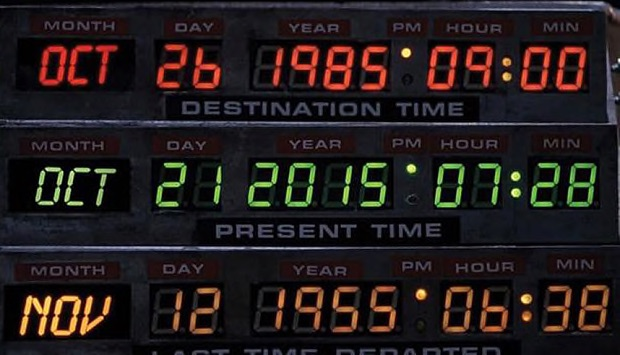
\includegraphics[height=2.5cm]{./img/bttf2.jpg}~
  
\includegraphics[height=2.5cm]{./img/rewind.jpg}~
  
\includegraphics[height=2.5cm]{./img/undo.jpg}\\

\includegraphics[height=2.4cm]{./img/undoredo.jpg}~
    
\includegraphics[height=2.4cm]{./img/tm.jpg}~
        
\includegraphics[height=2.4cm]{./img/debug.jpg} \\
                
\includegraphics[width=11cm]{./img/rever.jpg} 
\end{center}
\end{frame}

%%%% =======================================================

\begin{frame}
\frametitle{This Work}

%\begin{columns}[t]
%\column{.7\textwidth}
%\begin{enumerate}[$\bullet$]
	%\item 
	Reversible computation in models of message-passing concurrency, in particular process calculi
	
	\bigskip
	
	\textbf{Motivation:}
	\begin{enumerate}[$\bullet$]
	\item Rigorous basis for modern programming languages (Go, Erlang)
	\item Techniques based on type systems and contracts that enforce safety/liveness properties (``protocol conformance'')
	\item Programming abstractions that ``undo'' computation steps and return to a previous consistent state
	\item Analysis of workflow management systems with backward and forward ``jumps'' at runtime
	\end{enumerate}	
	
	\smallskip	
	%Key property: 
	\begin{tcolorbox}[%colback=gray!20,%gray background
                  colframe=black,% black frame colour
                  width=12.3cm,% Use 5cm total width,
                  arc=1.5mm, auto outer arc,left=1mm,right=1mm
                 ]
	\textbf{Causal consistency, Informally} (Danos \& Krivine, CONCUR'04): \\
	Reversibility doesn't lead to states not reachable with forward steps
\end{tcolorbox}
%	\item Communication-centric software: collections of communicating components that follow a global protocol (choreography)
%\end{enumerate}	

%\column{.3\textwidth}
%\centering
%aaaaaaaa
%\end{columns}

\end{frame}

%%%% =======================================================

\begin{frame}
\frametitle{Monitors-as-Memories Approach (JLAMP'17)}

%\begin{center}
\begin{tcolorbox}[colback=blue!5,%gray background
                  colframe=blue,% black frame colour
                  width=12.1cm,% Use 5cm total width,
                  arc=2mm, auto outer arc,
                 ]
\begin{center}
\textcolor{blue}{The \textbf{monitors} that verify protocol actions at runtime \\ \emph{used as} \\ the \textbf{memories} needed to reverse communication steps}
\end{center}
\end{tcolorbox}
%\end{center}

\bigskip
\textbf{Smooth integration of reversibility into interacting processes:}
	\begin{enumerate}[+]
	\item A monitor for each protocol participant, with a session type that describes the intended protocol
	\item A cursor in the type marks the protocol state: it moves forwards and backwards (reversing protocol actions)
	\item Streamlined proofs of causal consistency
	\end{enumerate}
	
\bigskip

\textbf{Shortcomings}:
	\begin{enumerate}[-]
	\item Only protocols between two partners (binary session types)
	\item Synchronous communication
	\end{enumerate}
\end{frame}

%%%% =======================================================

\begin{frame}
\frametitle{This Work: From Binary to Multiparty}
\begin{center}
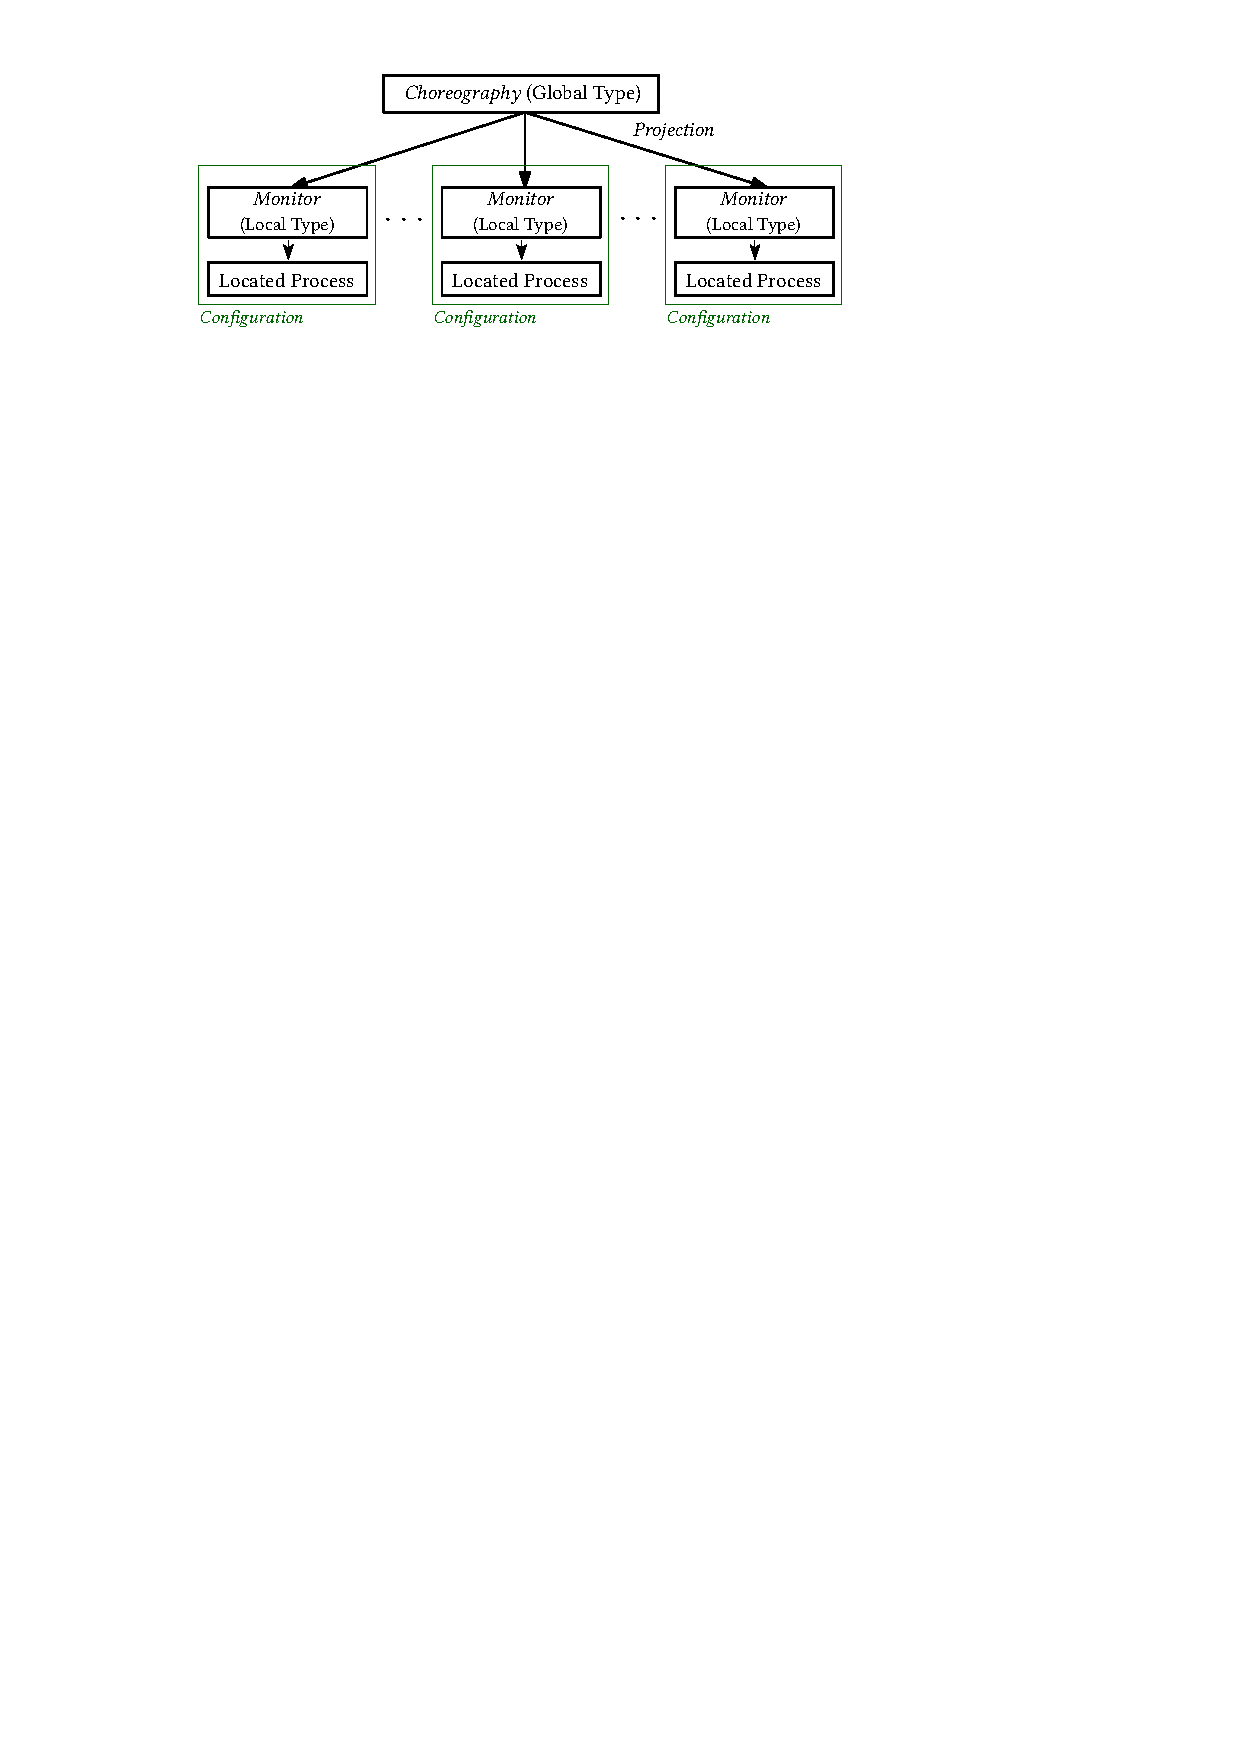
\includegraphics[scale=1.05]{figmodel}
\end{center}

\textbf{Highlights}:
\begin{enumerate}[$\bullet$]
%	\item Multiparty protocols
	\item Asynchronous communication, declaratively specified
	\item Higher-order process passing (name passing is representable!)
	\item Causal consistency 
	\end{enumerate}
\end{frame}

%%%% =======================================================

\begin{frame}
\frametitle{Technical Contributions}

%\textbf{In the paper:}
	\begin{enumerate}[1.]
	\item A new \textbf{process model} for reversible, multiparty sessions 
	\begin{enumerate}[$\bullet$]
	\item A concurrent $\lambda$-calculus with asynchronous process passing 
	\item Forward and backward  semantics for decoupled rollbacks 
	\item Monitors-as-memories approach extended to global types, local types, and their process implementations
	\end{enumerate}
	\item A proof of \textbf{causal consistency}
		\begin{enumerate}[$\bullet$]
	\item Needs an alternative semantics with \textbf{atomic rollbacks}, shown equivalent to the decoupled semantics
	\end{enumerate}	
	\item \textbf{Formal connection} of reversibility at two levels:
	\begin{enumerate}[$\bullet$]
	\item Declarative, given by global types 
	\item Operational, given by monitored processes
	\end{enumerate}
	\end{enumerate}	
	
	\smallskip
	\pause
	\begin{tcolorbox}[colback=red!10,%gray background
                  colframe=red,% black frame colour
                  width=12.2cm,% Use 5cm total width,
                  arc=1.5mm, auto outer arc,left=2mm,right=2mm,bottom=1mm,top=1mm,title=\textbf{In this talk}
                 ]
%\textbf{In this talk}: \\
The process model and causal consistency, by example.
\end{tcolorbox}
\end{frame}
%%%% =======================================================



%%%% =======================================================
%
%\begin{frame}
%\frametitle{Context and Motivation}
%
%Programming models for message-passing concurrency
%\begin{enumerate}[$\bullet$]
%	\item Processes communicate to exchange values, but also channels
%	\item Globally, a choreography declaratively describes the intended communication protocol between $n$ participants
%	\item Locally, a projection of the choreography onto each participant is used to govern process behavior, statically or dynamically
%\end{enumerate}
%
%\bigskip
%
%Reversible computation 
%\begin{enumerate}[$\bullet$]
%	\item Processes that ``undo'' some actions
%	\item A way of reacting to unforeseen circumstance (say, a local failure)
%	\item Forward and backwards operational semantics
%\end{enumerate}
%\end{frame}

%\part{The Process Model and Its Semantics}
%\frame{\partpage}

\section{The Process Model}

\begin{frame}
\frametitle{Governing Protocols: Global and Local Types}
\begin{center}
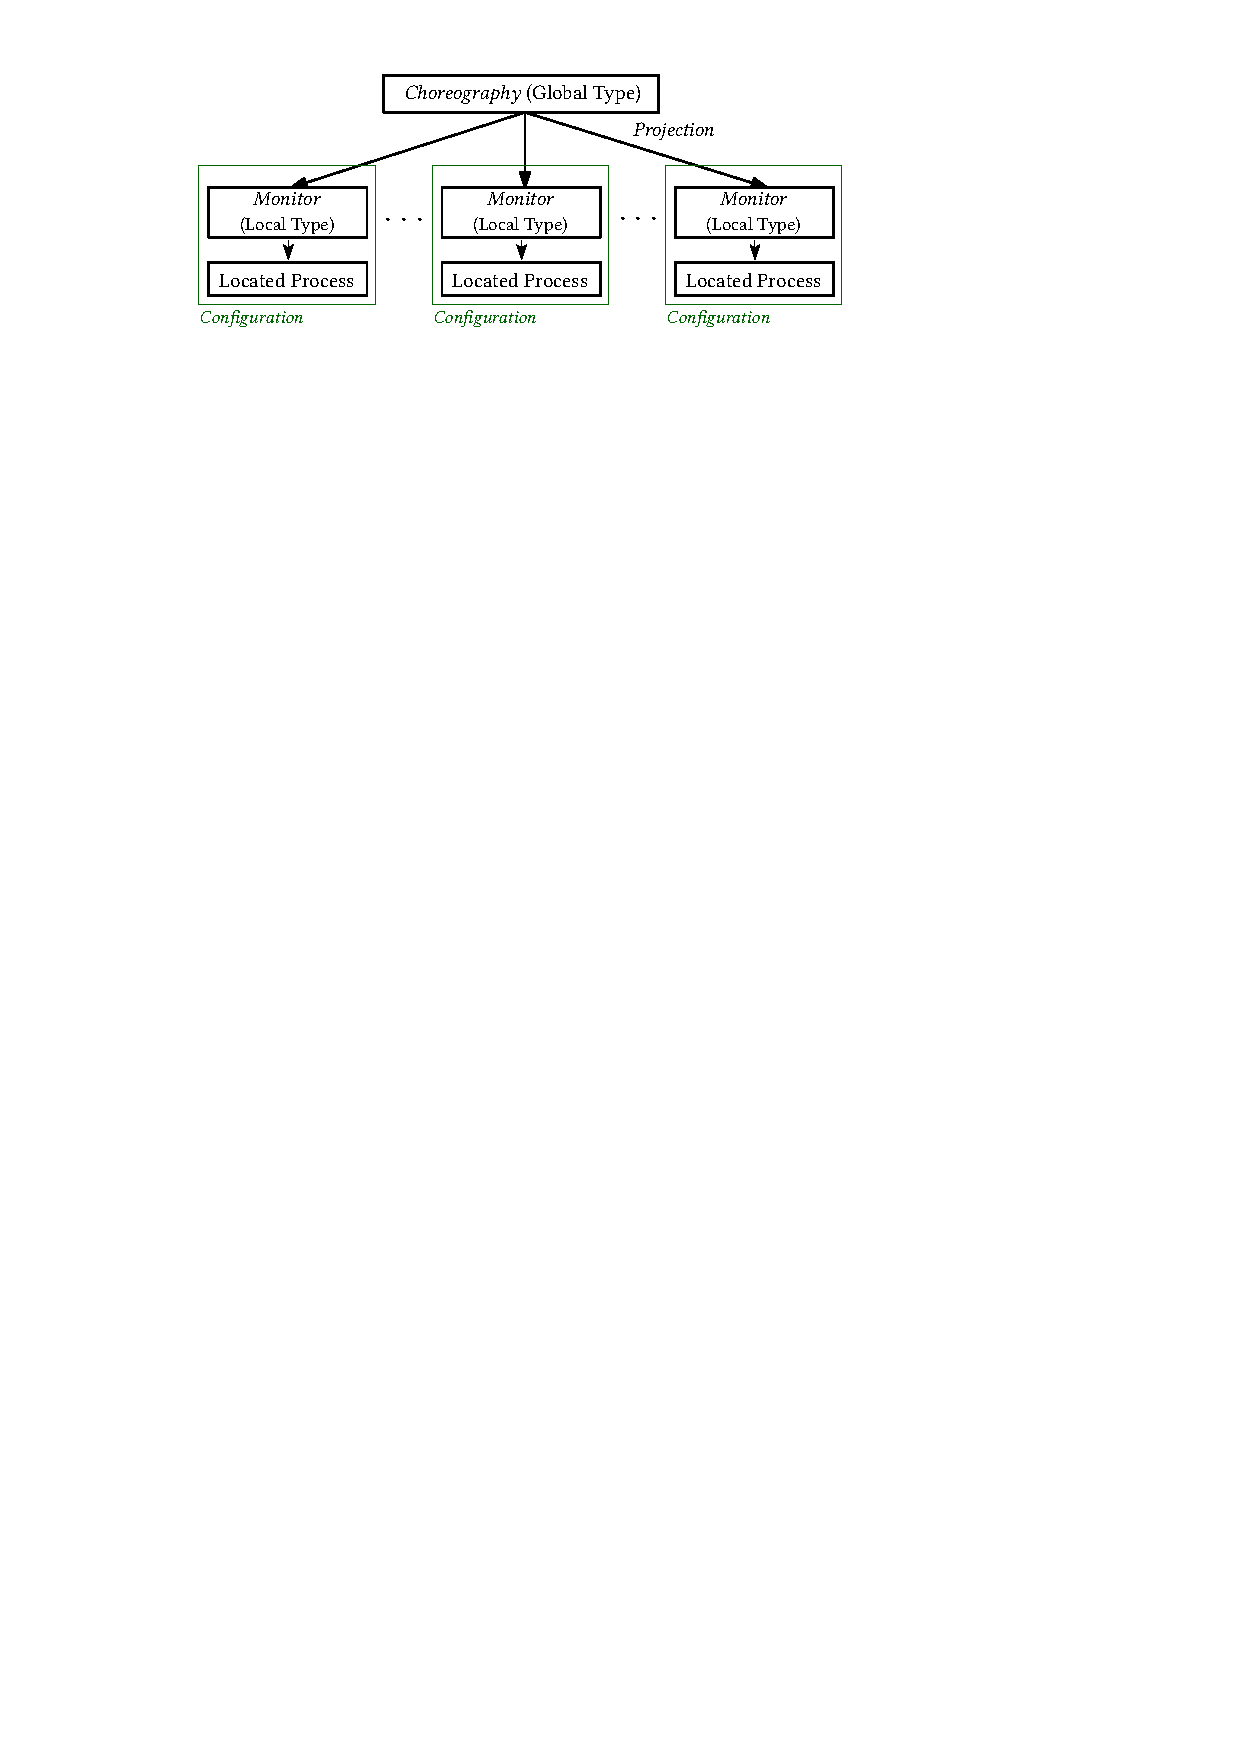
\includegraphics[scale=0.7]{figmodel}
\end{center}

\vspace{-8mm}
\begin{align*}
		\text{Global Types}~~	G, G'  \bnfis & \gtcom{p}{q}{U}{G} %\bnfbar 
			\sbnfbar %& 
			\mu X. G \sbnfbar X \sbnfbar \gend \\[-2.5mm]
		\text{Value Types}~~	U, U'  \bnfis & \bool \sbnfbar \nat \sbnfbar \cdots %\bnfbar T 
			\sbnfbar \sred{\rtsyn{\shot{T}}} \\[-2.5mm]
	    \text{Local Types}~~	T, T'  \bnfis & \ltout{p}{U}{T} \sbnfbar \ltinp{p}{U}{T} %\\
		  \sbnfbar %& 
		 \mu X. T \sbnfbar X \sbnfbar \lend 
\end{align*}

\bigskip
\textbf{Notice:}
\bi
\item $\shot{T}$ is the type of abstractions from names to processes
\item $\tproj{G}{\p}$ denotes the projection of $G$ onto participant $\p$ (standard)
\item Labelled choices can be easily incorporated (see our arXiv TR)
\ei
\end{frame}

\begin{frame}
\frametitle{Running Example: A Three-Buyer protocol }
\vspace{-2mm}
Alice (\pA), Bob (\pB), and Carol (\pC) interact with a Vendor (\pS):
\begin{align*}
G = ~&  \gtcom{A}{\pS}{\mathsf{title}}{~~\gtcom{\pS}{\{A,B\}}{\mathsf{price}}{\\[-0.5mm]
& \quad\gtcom{A}{B}{\mathsf{share}}{~~\gtcom{B}{\{A,\pS\}}{\mathsf{OK}}{
\\[-0.5mm]
& \quad\quad \gtcom{B}{C}{\mathsf{share}}{~~\gtcom{B}{C}{\textcolor{blue}{\thunkt}}{
\\[-0.5mm]
& \quad\qquad \gtcom{B}{\pS}{\mathsf{address}}{~~\gtcom{\pS}{B}{\mathsf{date}}{\gend}}}}}}}}
%\\
%G_2 = ~& \gtcom{B}{C}{\mathsf{share}}{\gtcom{B}{C}{T}{\gtcom{B}{C}{\shot{T}}{\gend}}}
\end{align*}
where $\textcolor{blue}{\thunkt}$ is the type of a \textbf{thunk process}:\\ % with type $\shot{\lend}$. 
Bob sends Carol some code with the protocol; she must activate it.

\bigskip
\pause 
Local types for the 
%The projection of $G$ onto the 
four participants (projections of $G$ onto $\pS, \pA, \pB, \pC$):
\begin{align*}
\tproj{G}{\pS} & = \ltinp{A}{\mathsf{title}\,}{\ltout{\{A,B\}}{\mathsf{price}}{\ltinp{B}{\mathsf{OK}}{\ltinp{B}{\mathsf{address}}{\ltout{B}{\mathsf{date}}{\lend}}}}}
\\
\tproj{G}{\pA} & = \ltout{\pS}{\mathsf{title}}{\ltinp{\pS}{\mathsf{price}}{\ltout{B}{\mathsf{share}}{\ltinp{B}{\mathsf{OK}}{\lend}}}}
\\
\tproj{G}{\pB} & = \ltinp{\pS}{\mathsf{price}}{\ltinp{A}{\mathsf{share}}{\ltout{\{A,\pS\}}{\mathsf{OK}}{
\\
& \qquad
\ltout{C}{\mathsf{share}}{\ltout{C}{\thunkt}{
 \ltout{\pS}{\mathsf{address}}{\ltinp{\pS}{\mathsf{date}}{\lend}}}}}}}
\\
\tproj{G}{\pC} & = \ltinp{B}{\mathsf{share}}{\ltinp{B}{\thunkt}{\lend}}
\end{align*}

\end{frame}

\begin{frame}
\frametitle{Key Ingredients}
\begin{enumerate}[$\bullet$]
\item  \textbf{Processes} $P, Q, \ldots$ include point-to-point value communication, recursion, and application 
\item  \textbf{Values} $V, W, \ldots$ include shared names and abstractions $\abs{x}{P}$. 
Name communication (delegation) can be represented.
\item  \textbf{Configurations} $M, N, \ldots$ are compositions of processes which are deployed in localities $\loc, \loc', \ldots$, one per participant $\p, \q, \ldots$
\pause
\item  There are also \textbf{run-time elements}, such as monitors and queues: they are configurations only generated at run-time
\item Monitors with local   types \textbf{with cursors}  $\mypast$:
		\begin{align*}
			    	T, T'  \bnfis & \ltout{p}{U}{T} \sbnfbar \ltinp{p}{U}{T}   \sbnfbar  
		 \mu X. T \sbnfbar X \sbnfbar \lend  \quad \text{\notas{as before}}\\[-2mm]
				\alpha \bnfis &   \typeIn{\q}{U} \sbnfbar  \typeOut{\q}{U} \\[-2mm]
	H,K		 \bnfis & \mypast T \sbnfbar T\mypast \sbnfbar \alpha_1.\cdots .\alpha_n.\mypast S 
	\end{align*}
		\\ (We need to add cursors also to global types; see the paper).
\end{enumerate}

% $H, H', \ldots$, which are protocol abstractions with a cursor $\past$
%\item  $\myloc{\loc}{\bout{a}{x}{P}}$ and $\myloc{\loc}{\binp{a}{x}{P}}$ denote the \emph{request} and \emph{acceptance}
%\item \emph{running processes} are of the form $\np{\ep{\loc}{\p}}{\conf{\stack C}{P}}$ 
%\item \emph{Monitors} are of the form $\monig{\ep{s}{\p}}{H}{\mytilde{x}}{\store}$ 
%\begin{itemize}
%	\item $\ep{s}{p}$ is the session endpoint
%	\item $H$ is  a session type with ``memory''
%	\item $\mytilde{x}$ is a set of free variables, 
%	\item $\store$  variables store
%\end{itemize}
%\item message queues of the form 
%$\codah{s}{h_i}{h_o}$, where $h_i$ is the past and $h_o$ the future

\end{frame}

\begin{frame}
	\frametitle{Syntax}
	\vspace{-9mm}
		\begin{align*}
\text{Names}~~ 					n,n' \bnfis & a,b \sbnfbar \ep{s}{\p}%, \dual{s} 
\qquad \quad
u,w  \bnfis n \sbnfbar x,y,z			
\\[-2mm]
%			\\
%			 {v},  {v}'  \bnfis &  \true \sbnfbar \false \sbnfbar \cdots
%			\\
	\text{Values}~~		V,W \bnfis & {a,b} \sbnfbar  x,y,z\sbnfbar {\abs{x}{P}}  \sbnfbar  \true \sbnfbar \false %v, v'
			\\[-2mm]
	\text{Processes}~~			P,Q
			 \bnfis &
			\bout{u}{V}{P}  \sbnfbar  \binp{u}{x}{P} 	\sbnfbar  
			 {\appl{V}{u}}  
			 %\\
			 %& 
			 \\[-2mm]
			  \sbnfbar & P \Par Q \sbnfbar  {\rvar{X} \sbnfbar \recp{X}{P}} 
			\sbnfbar \news{n} P \sbnfbar \inact
\\[-2mm]
\text{Configurations}~~M,N		 \bnfis &
\myloc{\loc}{\bout{a}{x:T}{P}}
\sbnfbar 
\myloc{\loc}{\binp{a}{x:T}{P}}
\\[-2mm]
\sbnfbar & 
M \Par N 
\sbnfbar 
\news{n} M
\sbnfbar 
\inact 
\\[-1mm]
 \sbnfbar &
\rtsyn{\np{\ep{\loc}{\p}}{\conf{\stack C}{P}}} %% running process
\\[-1mm]
\sbnfbar &
\rtsyn{\monig{\ep{s}{\p}}{H}{\mytilde{x}}{\store}}  %% monitor
\sbnfbar 
\rtsyn{\mem{k}{(\appl{V}{u})}{\loc}} % function
\\
 \sbnfbar &
\rtsyn{\codah{s}{h_i}{h_o}%{\restrict{\mytilde{\gpart{r}}}}
} % queue
%	\\
	  \\[-1.5mm]
\text{Queues}~~	 h \bnfis &  \emp   \sbnfbar h \cons \valueq{\p}{\q}{V}% \qquad m \bnfis V 
%\\
%\text{Tags}~~	\mytagg \bnfis & \rmark \sbnfbar \normark
%\qquad
%
 %   \alpha \bnfis &   \typeIn{\q}{U} \sbnfbar  \typeOut{\q}{U} 
  %  \\
%	T,S		 \bnfis & \lend \sbnfbar	\alpha.S 
%	\\
%	H,K		 \bnfis & \past T \sbnfbar T\past \sbnfbar \alpha_1.\cdots .\alpha_n.\past S 
%	\\
%	& 
\end{align*}
%\alpha \bnfis &   \typeIn{\q}{U} \sbnfbar  \typeOut{\q}{U} 
The tag $\mytagg$ can be $\rmark$ or $\normark$ if the monitor is involved in a rollback or not
\end{frame}

\subsection{Example (Part 1)}
\begin{frame}
\frametitle{Running Example: Process Implementations}

One process per protocol participant:
\begin{align*}
\text{Vendor} & =  \bout{d}{x:\tproj{G}{\pS}}\binp{x}{t}\bout{x}{price(t)}\bout{x}{price(t)}\\
& \qquad \binp{x}{ok}\binp{x}{a} \bout{x}{date}\inact  
\\
\text{Alice} & =  \binp{d}{y:\tproj{G}{\pA}}\bout{y}{\exBook}\binp{y}{p}\bout{y}{h}\binp{y}{ok}\inact  
\\
\text{Bob} & =  \binp{d}{z:\tproj{G}{\pB}}\binp{z}{p}\binp{z}{h}\bout{z}{ok}\bout{z}{ok}\bout{z}{h}
  \\
  & \qquad \qquad \bbout{z}{\textcolor{blue}{\thunkp{\bout{z}{\text{`Lucca, 55100'}}\binp{z}{d}\inact}}}\inact
  \\
\text{Carol} & =  \binp{d}{w:\tproj{G}{\pC}}\binp{w}{h}\binp{w}{\textcolor{blue}{code}}(\appl{\textcolor{blue}{code}}{\dummyn})
%&Q_B = \bout{y}{share}\bout{y}{T}\bout{y}{R}\inact  \\
%&Q_C = \binp{y}{share}\binp{y}{T}\binp{y}{X}\inact  \\
\end{align*}
where $\textcolor{blue}{\thunkp{P}}=\abs{x}{P}$, with $x \not \in fv(P)$, is a \textbf{thunk process}. \\
Upon activation of the thunk, received as $code$, Carol will send an address and receive a date on Bob's behalf.

\bigskip

A configuration results by placing these processes in four locations:
	$$M = \myloc{\loc_1}{\text{Vendor}} 
\Par
\myloc{\loc_2}{\text{Alice}} 
\Par
\myloc{\loc_3}{\text{Bob}} 
\Par 
\myloc{\loc_4}{\text{Carol}} 
$$
\end{frame}

\section{Semantics}
\begin{frame}
\frametitle{A  Monitor-based Session Semantics}
The binary case, as in
\notas{Kouzapas 2009; Hu et al, ECOOP'10}:
{\large 
\begin{mathpar}
\out{s}\msg{v}.P \Par
\only<2->{\textcolor{blue}{\bar{s}\queue{\send U.T_1 \cdot h_1}} \Par}
s(x).Q
\only<2->{\Par \textcolor{blue}{s\queue{\receive U.T_2 \cdot {h}_2}} }
\\
\only<3->{\rightarrow \\ 
P \Par
\uncover<4->{\textcolor{blue}{\bar{s}\queue{T_1 \cdot  {h}_1}}} \Par
Q
\uncover<4->{\Par \textcolor{blue}{s\queue{T_2 \cdot {h}_2,v}} }}
\end{mathpar}
}

\bi
\only<1->{\item Output and input processes along dual \textbf{endpoints} $\dual{s}$, $s$}
\only<2->{\item A monitor per endpoint (a type and a message queue $h_i$)}
%$\bar{s}\queue{\send U.S_1 \,\cdot\, \tilde{h}_1} $ is a \green{monitor} with session type $\send U.S_1$ and message queue $\tilde{h_1}$
\only<3->{\item Types enable synchronizations;} \only<4->{processes/types are \textbf{consumed}}
\ei

\end{frame}








\frame{
\frametitle{Our Idea: Cursors for Reversibility (JLAMP'17)}

{\large
\begin{mathpar}
\out{s}\msg{v}.P \Par 
\bar{s}\queue{\uncover<2->{\sred{\mypast}}\send U.T_1 \cdot h_1} \Par
s(x).Q
\Par s\queue{\uncover<2->{\sred{\mypast}}\receive U.T_2 \cdot {h}_2} 
\\
\only<3->{\fw \text{\notas{forward reduction}}\\ 
P \Par 
\bar{s}\queue{\send U.\sred{\mypast}T_1 \cdot h_1} \Par
Q
\Par
s\queue{\receive U.\sred{\mypast}T_2 \cdot {h}_2,v}}
\only<4->{ \\ \bk \text{\notas{backwards reduction}} \\
\out{s}\msg{v}.P \Par
\bar{s}\queue{\sred{\mypast}\send U.T_1 \cdot h_1}\Par
s(x).Q
\Par s\queue{\sred{\mypast}\receive U.T_2 \cdot {h}_2}
}
\end{mathpar}
}

\bi
\only<1->{\item Keep protocol information with a \textbf{cursor} on  types\only<2->{, written $\mypast$}}
\only<3->{\item The monitor allows us to move forward %($\fw$) 
\only<4->{and
backwards %($\bk$)
}}
\only<5->{\item Two operational semantics, denoted $\fw$ and $\bk$}
\ei
}

\begin{frame}
\frametitle{Forward Semantics ($\fw$): Key Ideas}
Our proposal for multiparty communication --- in five rules:
\bi
\item Session initiation checks that distributed participants implement compatible protocols, and sets up all the run-time machinery
\item Session communication is asynchronous, mediated by the queue, in two reduction steps \\
The types in the monitors have to enable these steps
\item $\beta$-reduction requires a special memory (``running function'') to record the exact part of the process where it occurs
\item Parallel composition is supporteds by splitting running processes
\ei
\end{frame}

\begin{frame}
	\frametitle{Forward Reduction  (1/5)}
	
	$$
	\infer [\fwcolor{(Init)}]
	{\parties{G}= \{\p_1,\cdots,\p_n\} \and \forall \gpart{p}_i\in \parties{G}. \, \tproj{G}{\gpart{p}_i} = T_{i}}
{
 {\begin{tabular}[b]{c}
 $\myloc{\loc_1}{\bout{a}{x_1:T_1}{P_{1}}} \Par \prod_{i \in \{2, \cdots, n\}}\myloc{\loc_i}{\binp{a}{x_i:T_i}{P_{i}}}$ 
  \\[1ex]
  \fw
  \\
  $\news{s} \large(\prod_{i \in\{1,\cdots,n\}} \np{\key{{\loc_{i}}}{\p_i}}{ \conf{\inact}{P_i\subst{\ep{s}{\p_i}}{x_i}}} 
  \Par \hmoni{\ep{s}{\p_i}}{\mypast T_{i}}{x_i}{\upd{x_i}{a }}$
  \\ 
$  \Par \codah{s}{\emp}{\emp}{})$
  \\
 \end{tabular}}
}
$$
%%\begin{mathpar}
%$$
%\infer[left=\fwcolor{(Init)}]
%{\parties{G}= \{\p_1,\cdots,\p_n\} \and 
%\forall \gpart{p}_i\in \parties{G}. \, \tproj{G}{\gpart{p}_i} = T_{i}  } 
%{ 
%\!\!\!\!
%\begin{tabular}[b]{cc}
%\myloc{\loc_1}{\bout{a}{x_1:T_1}{P_{1}}} \Par 
%\prod_{i \in \{2, \cdots, n\}}\myloc{\loc_i}{\binp{a}{x_i:T_i}{P_{i}}}  & 
%\\
%\fw &
%\news{s} \left(\, 
%\prod_{i \in\{1,\cdots,n\}} \np{\key{{\loc_{i}}}{\p_i}}{ \conf{\inact}{P_i\subst{\ep{s}{\p_i}}{x_i}}} \Par 
%\moni{\ep{s}{\p_i}}{\past T_{i}}{x_i}{\upd{x_i}{a }}  \Par \codah{s}{\emp}{\emp}{}\right)\!\!\!\!
%\end{tabular}
%}
%%\end{mathpar}
%$$
\vspace{-3mm}
\bi
\item One  request (at $\loc_1$) and $n-1$  accepts (at $\loc_2, \ldots, \loc_n$)
\item Reduction sets up the $n$-party session: fresh session names, running processes, monitors (with  tag $\normark$), and the empty queue
\item Cursors within the monitors are placed at the beginning
\ei
\end{frame}



\begin{frame}
	\frametitle{Forward Reduction  (2/5)}
$$
\infer*[left=\fwcolor{(Out)}]{
\p = \er \,\vee\, \p \in \names{\er, h_i}
}
{
{\begin{tabular}[b]{c}
$\np{\key{\loc}{\er}}{ \conf{\stack{C}}{\bout{\ep{s}{\p}}{V}{P}}} \Par \moni{\ep{s}{\p}}{\myctxr{\ctx{T}}{\mypast  \ltout{\q}{U}{S}}}{\mytilde x}{\store} 
$
 \\ 
 $\Par \codah{s}{h_i}{h_o}{} $
\\
\fw 
\\
$\np{\key{\loc}{\er}}{\conf{\stack{C}}{P}} \Par \moni{\ep{s}{\p}}{\myctxr{\ctx{T}}{ \ltoutp{\q}{U}{S}}}{\mytilde x}{\store}$ 
\\[1mm]
$\Par 
\codah{s}{h_i}{h_o\cons \valueq{\p}{\q}{\myeval{V}{\sigma}}}{}$
\end{tabular} 
}
}
$$
\vspace{-3mm}
\bi
\item $\ctx{T}$ is a type context (with past protocol actions)
\item Premise $\p = \er \,\vee\, \p \in \names{\er, h_i}$ allows performing actions on names previously received via abstraction-passing.
\ei
\end{frame}

\begin{frame}
	\frametitle{Forward Reduction  (3/5)}
$$
\infer*[left=\fwcolor{(In)}]{
\p = \er \,\vee\, \p \in \names{\er, h_i}
}
{
{\begin{tabular}[b]{c}
$\np{\key{\loc}{\er}}{\conf{\stack{C}}{\binp{\ep{s}{\p}}{y}{P}}} \Par \moni{\ep{s}{\p}}{\myctxr{\ctx{T}}{\mypast  \ltinp{\q}{U}{S}}}{\mytilde x}{\store}
$
 \\ 
 $\Par \codah{s}{h_i}{\valueq{\q}{\p}{V}\cons h_o }{}$
\\
\fw 
\\
$\np{\key{\loc}{\er}}{\conf{\stack{C}}{P}} \Par \moni{\ep{s}{\p}}{ \myctxr{\ctx{T}}{\ltinpp{\q}{U}{S}}}{\mytilde x, y}{\store\upd{y}{V}}$ 
\\[1mm]
$\Par \codah{s}{h_i\cons  \valueq{\q}{\p}{V}}{h_o }{} $
\end{tabular} 
}
}
$$
\vspace{-3mm}
\bi
\item The queue actually implements a history, separated by $\history$
\item $\ctx{T}$ is a type context (with past protocol actions)
\item Premise $\p = \er \,\vee\, \p \in \names{\er, h_i}$ allows performing actions on names previously received via abstraction-passing.
\ei
\end{frame}

 

\begin{frame}
	\frametitle{Forward Reduction  (4/5)}
%	\vspace{-5mm}
$$
\infer[\fwcolor{(Beta)}]{\myeval{V}{\sigma} =\abs{x}{P} }
{
{\begin{tabular}[b]{c}
$\np{\key{\loc}{\p}}{\conf{\stack{C}}{(\appl{V}{w})}} \Par \moni{\ep{s}{\p}}{\myctxr{\ctx{T}}{\mypast S}}{\mytilde x}{\store}$ 
\\
\fw 
\\
$\news{k}\, \left( {\np{\key{\loc}{\p}}{\conf{\ctx{\stack {C}}}{P\subst{\myeval{w}{\sigma}}{x}}}}  \Par \mem{k}{(\appl{V}{w})}{\loc} \Par\moni{\ep{s}{\p}}{\myctxr{\ctx T}{ k. \mypast S}}{\mytilde x}{\store} \right)$
\end{tabular}}
}
$$
\bi
\item A fresh $k$ is used in the running function and the monitor. 
\ei
\end{frame}	

\begin{frame}
	\frametitle{Forward Reduction  (5/5)}
$$
\infer*[left=\fwcolor{(Spawn)}]{  }
{
{\begin{tabular}[b]{c}
$\np{\key{\loc}{\p}}{\conf{\stack{C}}{P \Par Q}} \Par \moni{\ep{s}{\p}}{\myctxr{\ctx{T}}{\mypast S}}{\mytilde x}{\store}$
\\
\fw
\\
$\news{\loc_1,\loc_2}\, ( \np{\key{\loc}{\p}}{\conf{\stack{C}}{\inact}}  
\Par \np{\key{{\loc_1}}{\p}}{\conf{\inact}{P}}
\Par \np{\key{{\loc_2}}{\p}}{\conf{\inact}{Q}} 
$
\\[1mm]
$\Par \moni{\ep{s}{\p}}{\myctxr{\ctx T}{ (\loc,\loc_1,\loc_2). \mypast S}}{\mytilde x}{\store})
$
\end{tabular}}
}
$$

\bi
\item Location $\loc$ is split into running processes with fresh $\loc_1, \loc_2$.  \\
This is recorded in the monitor
\ei
\end{frame}	

\begin{frame}
\frametitle{Backward Semantics ($\bk$): Key Ideas}
\bi
\item The rollback of a synchronization is \textbf{decoupled}: \\
The two involved monitors are first jointly tagged (from $\normark$ to $\rmark$); then, each participant independently undoes its behavior
\item Undoing a forward session communication uses two backward reductions
\item Again, tagging and undoing steps have to be enabled by the type
\item In contrast, $\beta$-reductions and parallel processes are rollbacked atomically
\ei
\end{frame}

\begin{frame}
	\frametitle{Backward Semantics (1/2)}
	\vspace{-5mm}
$$
	\infer*[left=\bkcolor{(RollS)}]{ }{
	{\begin{tabular}[b]{c}
$\hmoni{\ep{s}{\p}}{ \myctxr{\ctx T}{\ltinpp{\q}{U}{T}}}{\mytilde x}{\store_1} $ 
\\[2mm]
$\Par \hmoni{\ep{s}{\q}}{ \myctxr{\ctx S}{\ltoutp{\p}{U}{S}}}{\mytilde y}{\store_2}$ 
%\codah{s}{h_i}{h_o}{\restrict{\mytilde{\gpart{r}}}}
\\[2mm]
$\Par \codah{s}{h_i}{h_o}{}$
\\
\bk 
\\
$\monir{\ep{s}{\p}}{ \myctxr{\ctx T}{\ltinpp{\q}{U}{T}}}{\mytilde x}{\store_1}$ 
\\
$\Par \monir{\ep{s}{\q}}{\myctxr{\ctx S}{\ltoutp{\p}{U}{S}}}{\mytilde y}{\store_2}$
%\codah{s}{h_i}{h_o}{\restrict{\mytilde{\gpart{r}},\p,\q}}
\\[2mm]
$\Par\codah{s}{h_i}{h_o}{}$
\end{tabular}}
}
$$
	\vspace{-5mm}
%	\pause
	\bi
\item Starts to undo a synchronization between $\p$ and $\q$ by \textbf{tagging} their monitors 
\item The two monitor types must be complementary
\item Once tagged, reversing input/output actions can occur independently
	\ei 
\end{frame}

%\begin{frame}
%	\frametitle{Backward semantics}
%	\begin{itemize}
%		\item we want to undo communication in a decouple way
%		\item monitors have to aggree
%	\end{itemize}	
%	\pause
%	\begin{mathpar}
%	{\scriptsize
%	\inferrule*[left=\bkcolor{(RollS)}]{ }{
%\hmoni{\ep{s}{\p}}{ \myctxr{\ctx T}{\ltinpp{\q}{U}{T}}}{\mytilde x}{\store_1} \Par 
%\hmoni{\ep{s}{\q}}{ \myctxr{\ctx S}{\ltoutp{\p}{U}{S}}}{\mytilde y}{\store_2} \Par 
%%\codah{s}{h_i}{h_o}{\restrict{\mytilde{\gpart{r}}}}
%\codah{s}{h_i}{h_o}{}
%\quad 
%\\
%\bk 
%\\
%\monir{\ep{s}{\p}}{ \myctxr{\ctx T}{\ltinpp{\q}{U}{T}}}{\mytilde x}{\store_1} \Par 
%\monir{\ep{s}{\q}}{\myctxr{\ctx S}{\ltoutp{\p}{U}{S}}}{\mytilde y}{\store_2} \Par 
%%\codah{s}{h_i}{h_o}{\restrict{\mytilde{\gpart{r}},\p,\q}}
%\codah{s}{h_i}{h_o}{}
%}}
%	\end{mathpar}
%	\pause
%	\begin{itemize}
%\item  starts to undo an input-output synchronization between $\p$ and $\q$ by \sred{\emph{preempting}} their monitors 
%\item two monitor types are complementary
%\item  undoing of input and output actions occurs in a decoupled way. 
%	\end{itemize} 
%\end{frame}



\begin{frame}
\frametitle{Backward Semantics (2/2)}
%\begin{mathpar}
%
%{%\scriptsize
%\inferrule*[left=\bkcolor{(RIn)}]{ 
%\p = \er \,\vee\, \p \in \names{\er, h_i}
%}
%{
%\np{\key{\loc}{\er}}{\conf{\stack C}{P}} \Par 
%\monir{\ep{s}{\p}}{ \myctxr{\ctx T} {\ltinpp{\q}{U}{S}} }{\mytilde x,y}{\store} \Par \\
%%\codah{s}{h_i\cons(\q,\p,V)}{h_o}{\restrict{\p,\mytilde{\gpart{r}}}}
%\codah{s}{h_i\cons(\q,\p,V)}{h_o}{}
%\\
%\quad \bk
%\\
%\np{\key{\loc}{\er}}{\conf{\stack C} { \binp{\ep{s}{\p}}{y}{P}} } \Par 
%\hmoni{\ep{s}{\p}}{ \myctxr{\ctx T}{\past\ltinp{\q}{U}{S}}}{\mytilde x}{\rup{\store}{y}}\Par \\ %\codah{s}{h_i}{(\q,\p,V)\cons h_o}{\restrict{\mytilde{\gpart{r}}}}
%\codah{s}{h_i}{(\q,\p,V)\cons h_o}{}
% }
% }
 
$$
\infer*[left=\bkcolor{(ROut)}]{\p = \er \,\vee\, \p \in \names{\er, h_i}
}{
{\begin{tabular}[b]{c}
$\np{\key{\loc}{\er}}{\conf{\stack C}{P}} \Par 
\monir{\ep{s}{\p}}{ \myctxr{\ctx T} {\ltinpp{\q}{U}{S}} }{\mytilde x,y}{\store} \Par 
$
\\
$\codah{s}{h_i\cons(\q,\p,V)}{h_o}{}$
 \\ 
 \bk 
 \\
$\np{\key{\loc}{\er}}{\conf{\stack C} { \binp{\ep{s}{\p}}{y}{P}} }
 \Par 
\hmoni{\ep{s}{\p}}{ \myctxr{\ctx T}{\past\ltinp{\q}{U}{S}}}{\mytilde x}{\rup{\store}{y}}\Par $
\\
$\codah{s}{h_i}{(\q,\p,V)\cons h_o}{}$
\end{tabular}}
}
$$


\bi
	\item Rule~\textsc{RIn} is symmetric to Rule~\textsc{In} and only enabled when the monitor is tagged as $\rmark$
	\item Other rules for $\bk$ are as expected
\ei

\end{frame}



%\begin{frame}
%\frametitle{Monitor-based Semantics  [Kouzapas et al.'10]}
%A sample reduction rule:
%{\large
%\begin{mathpar}
%\out{s}\msg{v}.P 
%\Par
%\overline{s}\queue{\send U.T_1 ; \tilde{h}_1} 
%\Par
%s(x).Q
%\Par
%s\queue{\receive U.T_2 ; \tilde{h}_2} 
%\\
%\longrightarrow 
%\\ 
%P \Par
%\overline{s}\queue{T_1 ; \tilde{h}_1} 
%\Par
%Q
%\Par
%s\queue{T_2 ; v \cdot \tilde{h}_2} 
%\end{mathpar}
%}
%
%\begin{enumerate}[$\bullet$]
%\item  $s(x).Q$ and $\out{s}\msg{v}.P$ and are I/O process along endpoints $\dual{s}$, $s$
%\item $\bar{s}\queue{\send U.S_1 ; \tilde{h}_1} $ is a \green{monitor} with session type $\send U.S_1$ and message queue $\tilde{h_1}$
%\end{enumerate}
%
%\end{frame}
%
%
%\begin{frame}
%\frametitle{Reversible hints}
%At each interaction the information of the type is lost: $\send U.S_1 \rightarrow S_1$
%	\begin{itemize}
%		\item we introduce session types with \green{present} and \green{past} $S\past T$ 
%	\end{itemize}
%	\vspace{.5cm}
%\begin{mathpar}
%\out{s}\msg{v}.P \parallel 
%\bar{s}\queue{\sred{\past}\send U.S_1 ; \tilde{h}_1} 
%\parallel
%s(x).Q
%\parallel
%s\queue{\sred{\past}\receive U.S_2 ; \tilde{h}_2} 
%\rightarrow \\ 
%P \parallel 
%\bar{s}\queue{ \send U.\sred{\past}S_1  ; \tilde{h}_1} 
%\parallel
%Q
%\parallel
%s\queue{\receive U.\sred{\past}S_2 ; v \cdot \tilde{h}_2} 
%\end{mathpar}
%\end{frame}
%
%\begin{frame}
%\frametitle{Aim}
%We are interested in studying reversibility in a setting where
%\begin{itemize}
%	\item Communications (e.g., message exchanges) among actors are well-disciplinated
%	\item Each participant has to obey to a protocol (e.g., behavioural type)
%	\item A monitor enforces a participant to follow its protocol
%	
%\end{itemize}
%\end{frame}
%
%\begin{frame}
%\frametitle{Background}
%	We build upon  previous work on binary synchronous session types
%	{\small
%	\begin{itemize}
%		\item  C. A. Mezzina and J. A. P\'erez. Reversibility in 
% session-based concurrency: A fresh look. J. Log. Algebr. Meth. Program., 90:2-30, 2017.
%		\item C. A. Mezzina and J. A. P\'erez. Reversible sessions using monitors. In D. A. Orchard and N. Yoshida, editors, PLACES 2016, volume 211 of EPTCS, pages 56-64, 2016.
%	\end{itemize}
%	}
%	
%	by considering
%	\begin{itemize}
%		\item multiparty session types
%		\item asynchrony
%		\item process passing
%	\end{itemize}
%\end{frame}
%
%\begin{frame}
%	\frametitle{Monitor as memory approach}
%	\begin{itemize}
%		\item Monitors are runtime entities that enact protocol actions
%		\item There exists a monitor for participant
%		\item the monitor contains information about the participant's type
%	\end{itemize}
%	
%\end{frame}
%
%
%
%
%\begin{frame}
%\frametitle{Model}
%\centering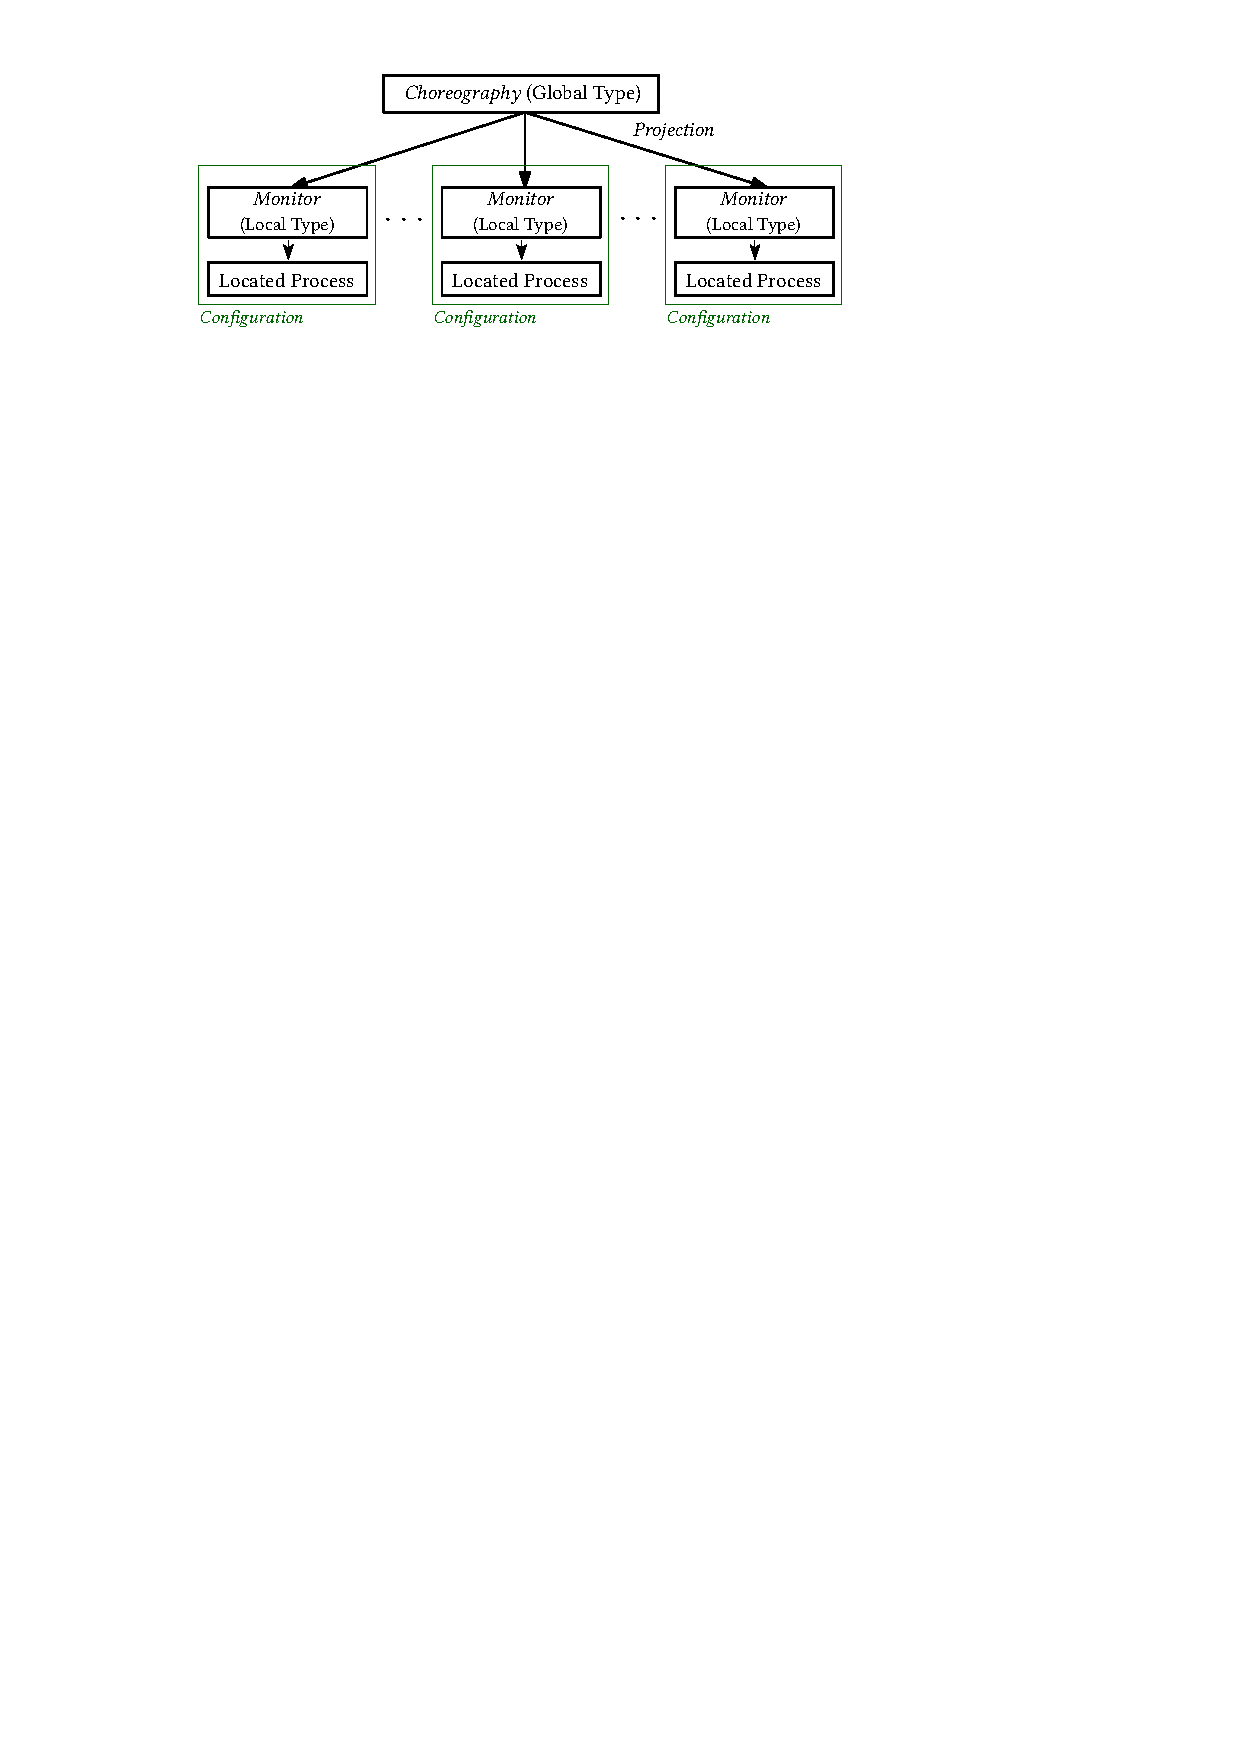
\includegraphics[scale=1]{figmodel}
%\end{frame}






%\begin{frame}
%\frametitle{Contents}
%\tableofcontents
%\end{frame}


\subsection{Example (Part 2)}
\begin{frame}
\frametitle{Running Example: The Semantics At Work}

Recall the configuration:
	$$M = \myloc{\loc_1}{\text{Vendor}} 
\Par
\myloc{\loc_2}{\text{Alice}} 
\Par
\myloc{\loc_3}{\text{Bob}} 
\Par 
\myloc{\loc_4}{\text{Carol}} 
$$
where processes are as follows:
\begin{align*}
\text{Vendor} & =  \bout{d}{x:\tproj{G}{\pS}}\binp{x}{t}\bout{x}{price(t)}\bout{x}{price(t)}\\
& \qquad \binp{x}{ok}\binp{x}{a} \bout{x}{date}\inact  
\\
\text{Alice} & =  \binp{d}{y:\tproj{G}{\pA}}\bout{y}{\exBook}\binp{y}{p}\bout{y}{h}\binp{y}{ok}\inact  
\\
\text{Bob} & =  \binp{d}{z:\tproj{G}{\pB}}\binp{z}{p}\binp{z}{h}\bout{z}{ok}\bout{z}{ok}\bout{z}{h}
  \\
  & \qquad \qquad \bbout{z}{\thunkp{\bout{z}{\text{`Lucca, 55100'}}\binp{z}{d}\inact}}\inact
  \\
\text{Carol} & =  \binp{d}{w:\tproj{G}{\pC}}\binp{w}{h}\binp{w}{code}(\appl{code}{\dummyn})
%&Q_B = \bout{y}{share}\bout{y}{T}\bout{y}{R}\inact  \\
%&Q_C = \binp{y}{share}\binp{y}{T}\binp{y}{X}\inact  \\
\end{align*}
%\centering{\blue{$\thunkp{P} =\abs{x}{P}$ with $x \not \in \fn{P}$}}
Let's examine some forward and backward reductions from $M$. 

\end{frame}

\begin{frame}
	\frametitle{Forward Semantics: Session Initialization}
	$$M = \myloc{\loc_1}{\text{Vendor}} 
\Par
\myloc{\loc_2}{\text{Alice}} 
\Par
\myloc{\loc_3}{\text{Bob}} 
\Par 
\myloc{\loc_4}{\text{Carol}} 
$$

	\begin{align*}
%\begin{array}{cc}
M & \fw  \news{s}\big(\, 
\np{\key{{\loc_1}}{\pS}}{ \conf{\inact}{V_1\subst{\epS}{x}}} \Par 
\hmoni{\ep{s}{\pS}}{\mypast \tproj{G}{\pS}}{x}{\upd{x}{d}}  
\\
& \Par \np{\key{{\loc_2}}{\pA}}{ \conf{\inact}{A_1\subst{\epA}{y}}} \Par 
\hmoni{\ep{s}{\pA}}{\mypast \tproj{G}{\pA}}{y}{\upd{y}{d}} 
\\
& \Par \np{\key{{\loc_3}}{\pB}}{ \conf{\inact}{B_1\subst{\epB}{z}}} \Par 
\hmoni{\ep{s}{\pB}}{\mypast \tproj{G}{\pB}}{z}{\upd{z}{d}} 
\\
& \Par \np{\key{{\loc_4}}{\pC}}{ \conf{\inact}{C_1\subst{\epC}{w}}} \Par 
\hmoni{\ep{s}{\pC}}{\mypast \tproj{G}{\pC}}{w}{\upd{w}{d}}  
\\
& \Par \codah{s}{\emp}{\emp}{}~\big)  = M_1
%\end{array}
\end{align*}
\bi
	\item Each monitor type is initialized with $\mypast$
	\item A queue with empty memory is created
	\item At this point we could either undo the initialization, or proceed further with the protocol
\ei
\end{frame}

\begin{frame}
\frametitle{Forward Semantics: Asynchronous Output}

The first action of Alice is to send $\exBook$ to Vendor:
\begin{align*}
M_1 & \fw  \news{s}(\,  \np{\key{{\loc_2}}{\pA}}{ \conf{\inact}{\binp{\epA}{p}\bout{\epA}{h}\binp{\epA}{ok}\inact}} 
\\
& \!\!\!\!\Par 
\hmoni{\ep{s}{\pA}}{\ltout{\pS}{\mathsf{title}}{\mypast \ltinp{\pS}{\mathsf{price}}{\ltout{B}{\mathsf{share}}{\ltinp{B}{\mathsf{OK}}{\lend}}}}}{y}{\upd{y}{d}} 
\\
& \!\!\!\!\Par N_2 \Par \codah{s}{\emp}{\valueq{\pA}{\pS}{\exBook}}{}~) = M_2\\
 \fw  \\
\uncover<2->{&\!\!\!\!\news{s}(\,  \np{\key{{\loc_1}}{\pS}}{ \conf{\inact}{\bout{\epS}{price(t)} \bout{\epS}{price(t)}\binp{\epS}{ok}\\ 
& \qquad  \binp{\epS}{a} \bout{\epS}{date}\inact }} 
\\
& \Par 
\hmoni{\ep{s}{\pS}}{\ltinp{A}{\mathsf{title}}{\mypast \ltout{\{A,B\}}{\mathsf{price}}{T_\pS}}}{x,t}{\store_3}  \Par N_3
\\
&  \Par \codah{s}{\valueq{\pA}{\pS}{\exBook}}{\emp}{}~) = M_3} 
\end{align*}
\uncover<3->{In $M_3$ we have: 
\bi
%\item $N_i$ stand for the rest of the system
\item $\store_3  = \upd{x}{d},\upd{t}{\exBook}$ is the resulting store
\item $T_\mathsf{\pS}  = \ltinp{B}{\mathsf{OK}}{\ltinp{B}{\mathsf{address}}{\ltout{B}{\mathsf{date}}{\lend}}}$
%and $N_3$ stands for the participants not involved in the reduction.
%Observe that 
%\item the cursors in monitors $\ep{s}{\pS}$ and $\ep{s}{\pA}$ have evolved, and that 
\item the message from $\pA$ to $\pS$ has now been moved to the input queue
\ei
}
\end{frame}

\begin{frame}
\frametitle{Decoupled Rollback (1/3)}
Returning to $M_1$ starting from $M_3$. \\
We need to apply Rules~\bkcolor{\textsc{(RollS)}}, \bkcolor{\textsc{(RIn)}}, and \bkcolor{\textsc{(ROut)}}.
\begin{align*}
M_3 & \bk  \news{s}(\,  
\np{\key{{\loc_1}}{\pS}}{ \conf{\inact}{\bout{\epS}{price(t)}\bout{\epS}{price(t)}\binp{\epS}{ok} \\ 
& \quad  \binp{\epS}{a} \bout{\epS}{date}\inact }} 
\\
& \Par 
 \monir{\ep{s}{\pS}}{\ltinp{A}{\mathsf{title}}{\mypast \ltout{\{A,B\}}{\mathsf{price}}{T_\mathsf{B}}}}{x,t}{\store_3} 
\\
& \Par \np{\key{{\loc_2}}{\pA}}{ \conf{\inact}{\binp{\epA}{p}\bout{\epA}{h}\binp{\epA}{ok}\inact}} 
\\
& \Par 
\monir{\ep{s}{\pA}}{\myctxr{\ctx{T}_4}{\mypast \ltinp{\pS}{\mathsf{price}}{\ltout{B}{\mathsf{share}}{\ltinp{B}{\mathsf{OK}}{\lend}}}}}{y}{\upd{y}{d}} 
\\
& \Par N_4 \Par \codah{s}{\valueq{\pA}{\pS}{\exBook}}{\emp}{}~)  = M_4
\end{align*}
Notice:
\bi
\item By applying \bkcolor{\textsc{(RollS)}} monitors for \pS and \pA have now tag $\rmark$
\item In the monitor for \pA, we have $\myctxr{\ctx{T}_4}{\bullet}  =\ltout{\pS}{\mathsf{title}}{\bullet}$ 
\item $M_4$ has several possible forward and backward reductions.
\ei
\end{frame}

\begin{frame}
\frametitle{Decoupled Rollback (2/3)}
Using Rule~\bkcolor{\textsc{(RIn)}} to first undo the input at \pS:
\begin{align*}
M_4 & \bk  \news{s}(\,  
\np{\key{{\loc_1}}{\pS}}{ \conf{\inact}{\binp{\epS}{t}\bout{\epS}{price(t)}\bout{\epS}{price(t)} \\ 
& \quad  \binp{\epS}{ok}\binp{\epS}{a} \bout{\epS}{date}\inact }} 
\\
& \Par 
 \hmoni{\ep{s}{\pS}}{\mypast \ltinp{A}{\mathsf{title}}{\ltout{\{A,B\}}{\mathsf{price}}{T_\mathsf{B}}}}{x}{\upd{x}{d}} 
\\
& \Par \np{\key{{\loc_2}}{\pA}}{ \conf{\inact}{\binp{\epA}{p}\bout{\epA}{h}\binp{\epA}{ok}\inact}} 
\\
& \Par 
\monir{\ep{s}{\pA}}{\myctxr{\ctx{T}_4}{\mypast \ltinp{\pS}{\mathsf{price}}{\ltout{B}{\mathsf{share}}{\ltinp{B}{\mathsf{OK}}{\lend}}}}}{y}{\upd{y}{d}} 
\\
& \Par N_4 \Par \codah{s}{\emp}{\valueq{\pA}{\pS}{\exBook}}{}~)  = M_5
\end{align*}
\bi
\item The input at $\pS$ has been undone, as witnessed by the modified cursor and tag $\normark$
\item The output at $\pA$ still needs to be reversed (hence the tag $\rmark$); this can take place from $M_5$ at any time 
\ei
\end{frame}

\begin{frame}
\frametitle{Decoupled Rollback (3/3)}
A particular reduction from $M_5$ undoes the output at \pA:
\begin{align*}
M_5 & \bk  \news{s}(\,  
\np{\key{{\loc_1}}{\pS}}{ \conf{\inact}{\binp{\epS}{t}\bout{\epS}{price(t)}\bout{\epS}{price(t)} \\ 
&   \binp{\epS}{ok}\binp{\epS}{a} \bout{\epS}{date}\inact }} 
\\
&  \!\!\!\! \Par 
 \hmoni{\ep{s}{\pS}}{\!\!\mypast \ltinp{A}{\mathsf{title}}{\ltout{\{A,B\}}{\mathsf{price}}{T_\mathsf{B}}}}{x}{\upd{x}{d}} 
\\
& \!\!\!\! \Par \np{\key{{\loc_2}}{\pA}}{ \conf{\inact}{\bout{\epA}{\exBook}\binp{\epA}{p}\bout{\epA}{h}\binp{\epA}{ok}\inact}} 
\\
& \!\!\!\!\Par 
\hmoni{\ep{s}{\pA}}{\!\!\mypast \ltout{\pS}{\mathsf{title}}{\ltinp{\pS}{\mathsf{price}}{\ltout{B}{\mathsf{share}}{\ltinp{B}{\mathsf{OK}}{\lend}}}}}{y}{\upd{y}{d}} 
\\
& \!\!\!\! \Par N_4 \Par \codah{s}{\emp}{\emp}{}~)  = M_6
\end{align*}

\bi
\item Clearly, $M_6 = M_1$.
\item Summing up, the synchronization realized by \\ the   sequence
$M_1 \fw M_2 \fw M_3$ can be reversed by \\ the    sequence
$M_3 \bk M_4 \bk M_5 \bk M_6$
\ei
\end{frame}

\begin{frame}
\frametitle{Forward Abstraction Passing (1/3)}
\vspace{-1.5mm}
Assume that $M_3$ follows a sequence of forward reductions
until $M_7$:
\begin{align*}
M_7 = ~ &   \news{s}(\,  \np{\key{{\loc_3}}{\pB}}{ \conf{\inact}{\bbout{\epB}{\thunkp{\bout{\epB}{\text{`Lucca, 55100'}}\binp{\epB}{d}\inact}}\inact}} 
\\
& \!\!\!\! \Par \hmoni{\ep{s}{\pB}}{\myctxr{\ctx{T}_7}{\mypast \ltout{C}{\thunkt}{\ltout{\pS}{\mathsf{address}}{\ltinp{\pS}{\mathsf{date}}{\lend}}}}}{z,p,h}{\store_7} 
\\[2mm]
& \!\!\!\! \Par \np{\key{{\loc_4}}{\pC}}{ \conf{\inact}{\binp{\epC}{code}(\appl{code}{\dummyn})}} 
\\
&  \!\!\!\! \Par 
\hmoni{\ep{s}{\pC}}{\myctxr{\ctx{T}_8}{\mypast \ltinp{B}{\thunkt}{\lend}}}{w,h}{\store_8} 
\Par N_5 \Par \codah{s}{h_7}{\emp}{}~) 
\end{align*}
\smallskip
\pause
where 
$\myctxr{\ctx{T}_7}{\bullet}$, $\store_7$, $\myctxr{\ctx{T}_8}{\bullet}$, $\store_8$,
and $h_7$ capture prior steps as follows:
\begin{align*}
\myctxr{\ctx{T}_7}{\bullet} & =
\ltinp{\pS}{\mathsf{price}}{\ltinp{A}{\mathsf{share}}{\ltout{\{A,\pS\}}{\mathsf{OK}}{
\ltout{C}{\mathsf{share}}{\bullet}}}}
\\
\store_7 & = \upd{z}{d},\upd{p}{price(\exBook)},\upd{h}{120}
\\
\myctxr{\ctx{T}_8}{\bullet} & =\ltinp{B}{\mathsf{share}}{\bullet} \qquad \store_8  = \upd{w}{d},\upd{h}{120}
\\
h_7 & = 
\valueq{\pA}{\pS}{\exBook}
\\
& \cons
\valueq{\pS}{\pA}{price(\exBook)}
\cons
\valueq{\pS}{\pB}{price(\exBook)}
\\
& \cons
\valueq{\pA}{\pB}{120}
\cons
\valueq{\pB}{\pA}{\text{`ok'}}
\cons
\valueq{\pB}{\pS}{\text{`ok'}}
\cons
\valueq{\pB}{\pC}{120}
\end{align*}
\end{frame}

\begin{frame}
\frametitle{Forward Abstraction Passing (2/3)}

If $M_7 \fw \fw M_8$ by using Rules~\fwcolor{\textsc{(Out)}} and~\fwcolor{\textsc{(In)}}, then
we would have a higher-order communication:
\begin{align*}
M_8 & = ~   \news{s}(\,  \np{\key{{\loc_3}}{\pB}}{ \conf{\inact}{\inact}} 
\\
& \Par \hmoni{\ep{s}{\pB}}{\myctxr{\ctx{T}_7}{\ltout{C}{\thunkt}{\mypast\ltout{\pS}{\mathsf{address}}{\ltinp{\pS}{\mathsf{date}}{\lend}}}}}{z,p,h}{\store_7} 
\\
& \Par \np{\key{{\loc_4}}{\pC}}{ \conf{\inact}{(\appl{code}{\dummyn}) }} 
\\
& \Par 
\hmoni{\ep{s}{\pC}}{\myctxr{\ctx{T}_8}{ \ltinp{B}{\thunkt}{\mypast\lend}}}{w,h,code}{\store_9} 
\\
& 
\Par N_5 \Par \codah{s}{h_7 \cons \valueq{\pB}{\pC}{\thunkp{\bout{\epB}{\text{`Lucca, 55100'}}\binp{\epB}{d}\inact}}}{\emp}{}~) 
\end{align*}
where
$\store_9 = \store_8 \upd{code}{\thunkp{\bout{\epB}{\text{`Lucca, 55100'}}\binp{\epB}{d}\inact}}$.

\end{frame}

\begin{frame}
\frametitle{Forward Abstraction Passing (3/3)}
We may apply Rule~\fwcolor{\textsc{(Beta)}} to obtain the code sent from \pB to \pC:
\begin{align*}
M_8 & \fw ~   \news{s}\news{k}(\,  
%\np{\key{\loc_3}{\pB}}{ \conf{\inact}{\inact}} 
%\\
%& \Par \hmoni{s_\pB}{\myctxr{\ctx{T}_7}{\ltout{C}{\thunkt}{\past\ltout{S}{\mathsf{address}}{\ltinp{S}{\mathsf{date}}{\lend}}}}}{z,p,s}{\store_7} 
%\\
%& \Par 
\np{\key{{\loc_4}}{\pC}}{\conf{\inact}{\bout{\epB}{\text{`Lucca, 55100'}}\binp{\epB}{d}\inact}} 
\!\!  \Par N_6 
\\
& \!\!\Par \hmoni{\ep{s}{\pB}}{\myctxr{\ctx{T}_7}{\ltout{C}{\thunkt}{\mypast\ltout{\pS}{\mathsf{address}}{\ltinp{\pS}{\mathsf{date}}{\lend}}}}}{z,p,h}{\store_7} 
\\
& \!\!\Par 
\mem{k}{(\appl{code}{\dummyn})}{{\loc_4}} 
\Par 
\hmoni{\ep{s}{\pC}}{\myctxr{\ctx{T}_8}{ \ltinp{B}{\thunkt}{k.\mypast\lend}}}{w,h,code}{\store_9} 
\\
& 
\!\!\Par \codah{s}{h_7 \cons \valueq{\pB}{\pC}{\thunkp{\bout{\epB}{\text{`Lucca, 55100'}}\binp{\epB}{d}\inact}}}{\emp}{}~) 
= M_9
\end{align*}
%where $N_6$ is for the rest of the system. 
\vspace{-3mm}
\bi
\item This reduction added a running function on a fresh 
$k$, which is also used within the monitor $\ep{s}{\pC}$.

\item Reduction $M_8 \fw M_9$ completes the code mobility from $\pB$ to $\pC$: the now active thunk
will run $\pB$'s implementation from $\pC$'s location. 
\item Observe that Bob's identity \pB is ``hardwired'' in the sent thunk. 
%there is no way for \pC to execute the code by referring to a participant different  from \pB.
This justifies the premise 
$\p = \er \,\vee\, \p \in \names{\er, h_i}$.
% present in Rules~\fwcolor{\textsc{(Out)}} and \fwcolor{\textsc{(In)}}  (and in their backward counterparts).
%when executing previously received mobile code, the participant mentioned in the location (i.e., $\pC$) and that mentioned in the located process (i.e., $\pB$) may differ.
\item Reductions from $M_9$ will  modify the cursor in the type stored in monitor $\ep{s}{\pB}$
based on the process located at $\key{{\loc_4}}{\pC}$.
\ei
\end{frame}

%\begin{frame}
%\frametitle{-}
%\bi
%\item -
%\ei
%\end{frame}
%
%\begin{frame}
%\frametitle{-}
%\bi
%\item -
%\ei
%\end{frame}

\section{Causal Consistency}

\newcommand{\trace}{\rho}
\newcommand{\etrace}{\varepsilon}

\newcommand{\causeq}{\asymp}
\newcommand{\nottrace}[1]{{#1}_\bullet}
\newcommand{\tsource}[1]{\mathtt{src}(#1)}
\newcommand{\ttarget}[1]{\mathtt{trg}(#1)}


\begin{frame}
	\frametitle{Causal Consistency (1/3)}
	
%	Intuitively, causal consistency ensures that
%	\bi
%	\item Reversible steps lead to system states that could been have reached by performing forward steps only. 
%	\item That is, causally consistent reversibility does not lead to extraneous states, not reachable through ordinary computations.
%	\ei
	
	Intuitively, causal consistency characterizes rollbacks which are:
	\bi
		\item \textbf{Consistent}: do not lead to past unreachable configurations
		\item \textbf{Flexible}: admit the rearrangement of reversed actions
		%This may enable us to obtain rollback sequences more efficient than those decreeing the naive reversal of each performed step.
		\ei
Thus, the set of states reached by a backward step could have been reached by performing only forward computations.
	
	\bigskip
	\pause
	
	Causal consistency is a property of \textbf{traces of transitions} between configurations.
	\textbf{Causal equivalence} $\causeq$ ensures:
	\bi
	\item given two \emph{concurrent} transitions, the traces obtained by swapping their execution order are equivalent
	\item a trace consisting of opposing transitions is equivalent to the empty trace
	\ei
	
%	\smallskip
%	
%	\begin{theorem}[Causal consistency]\label{t:causal}
% Let $\trace_1$ and $\trace_2$ be coinitial traces of transitions. \\
% Then 
% $\trace_1 \causeq \trace_2$ if and only if $\trace_1$ and $\trace_2$ are cofinal.
%\end{theorem}


\end{frame}
\begin{frame}
	\frametitle{Causal Consistency (2/3)}
	The flexibility of the decoupled semantics makes proving \textbf{causal consistency} difficult
	\bi
		\item We move to a synchronous semantics with atomic rollbacks and communications (``atomic semantics'')
		\item The decoupled and atomic semantics are tightly related via \\
		(1)~a bi-directional operational correspondence and \\
		(2)~a back-and-forth barbed bisimilarity
		\item It then suffices to prove causal consistency on the atomic semantics!
	\ei
\end{frame}

\begin{frame}
	\frametitle{Causal Consistency (3/3)}
	\vspace{-3mm}
	\begin{theorem}[Causal consistency]\label{t:causal}
 Let $\trace_1$ and $\trace_2$ be coinitial traces of transitions. \\
 Then 
 $\trace_1 \causeq \trace_2$ if and only if $\trace_1$ and $\trace_2$ are cofinal.
\end{theorem}

	We follow the ``recipe'' by Danos \& Krivine, using three  lemmas:
\begin{figure}[!t]
    \centering
    \begin{subfigure}[b]{3.7cm}
    \centering
        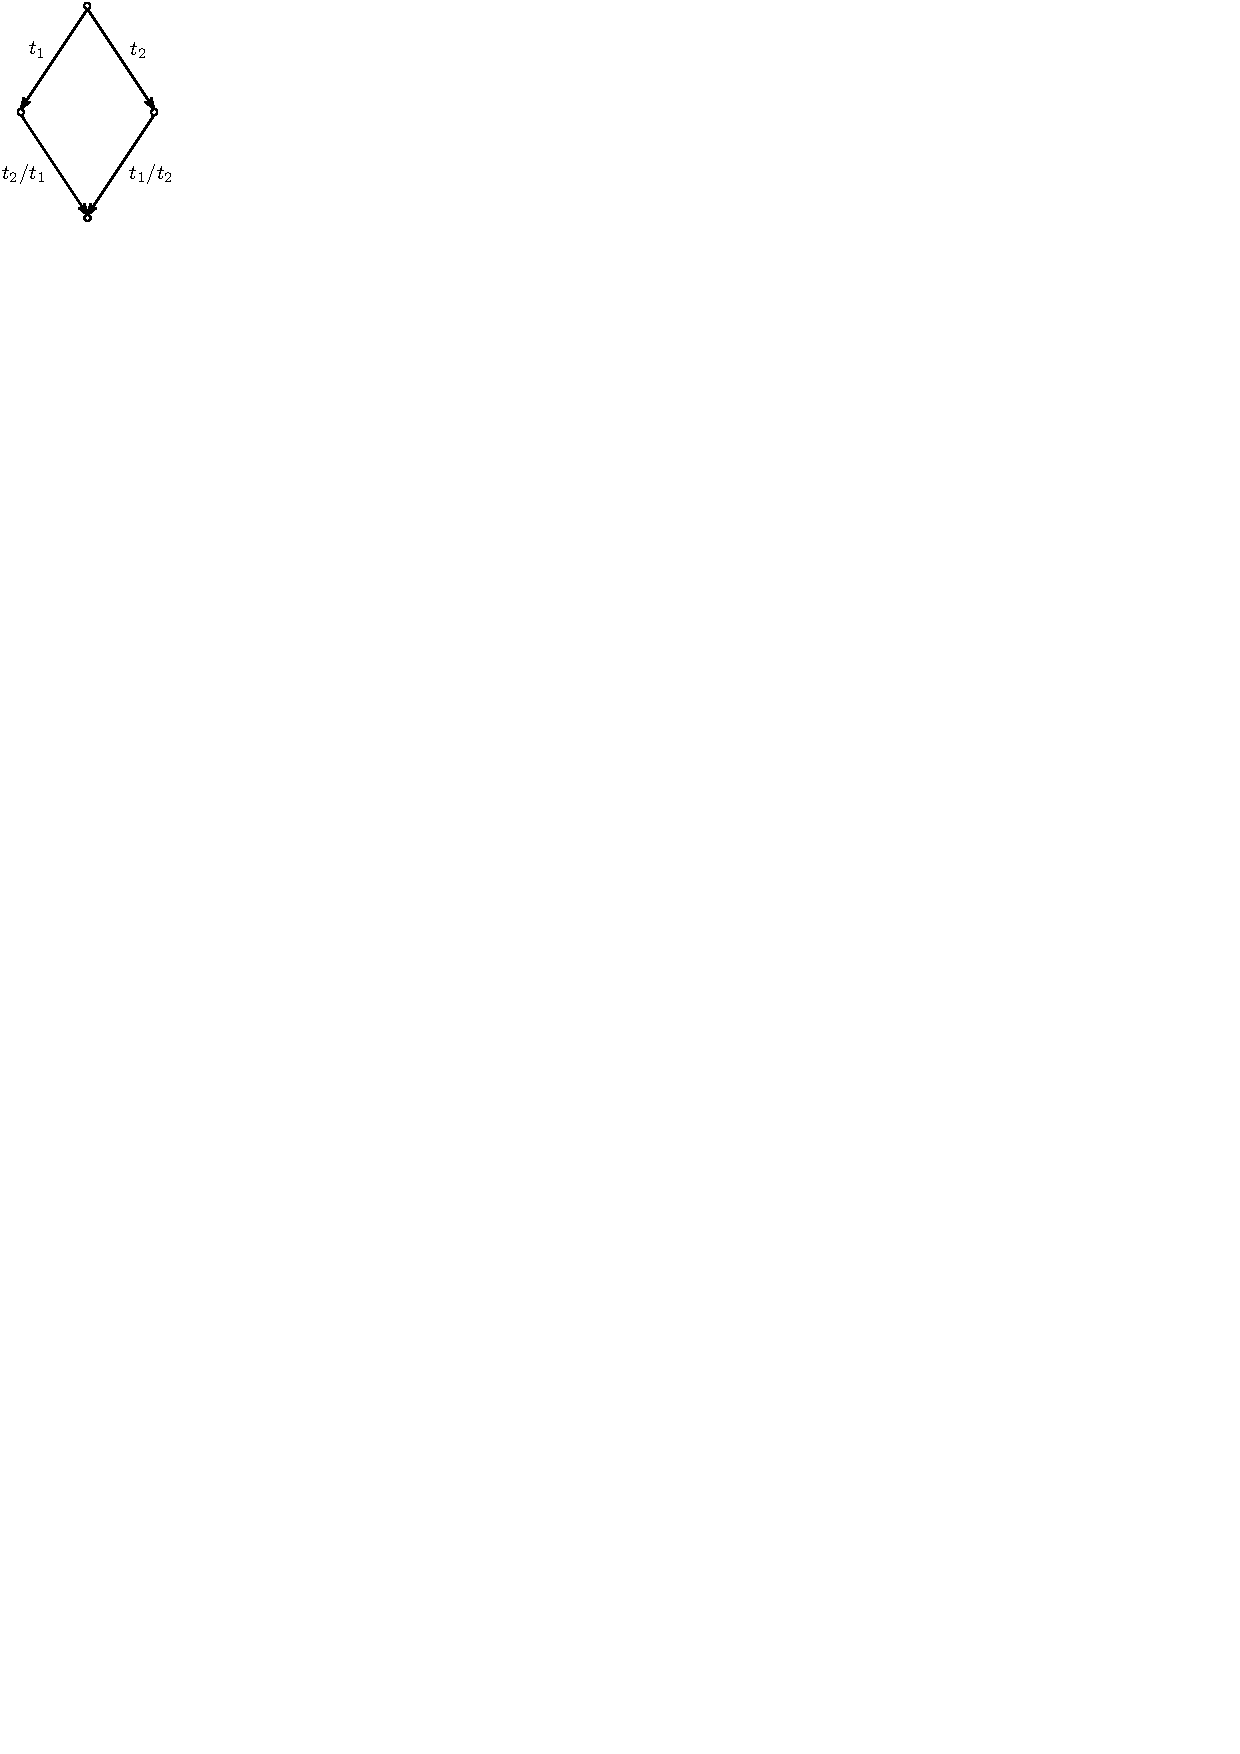
\includegraphics[height=3.5cm]{./img/square}
        \caption{Square Lemma %\\ (Lemma~\ref{lm:square})
        }
        \label{fig:square}
    \end{subfigure}
        \begin{subfigure}[b]{3.9cm}
        \centering
        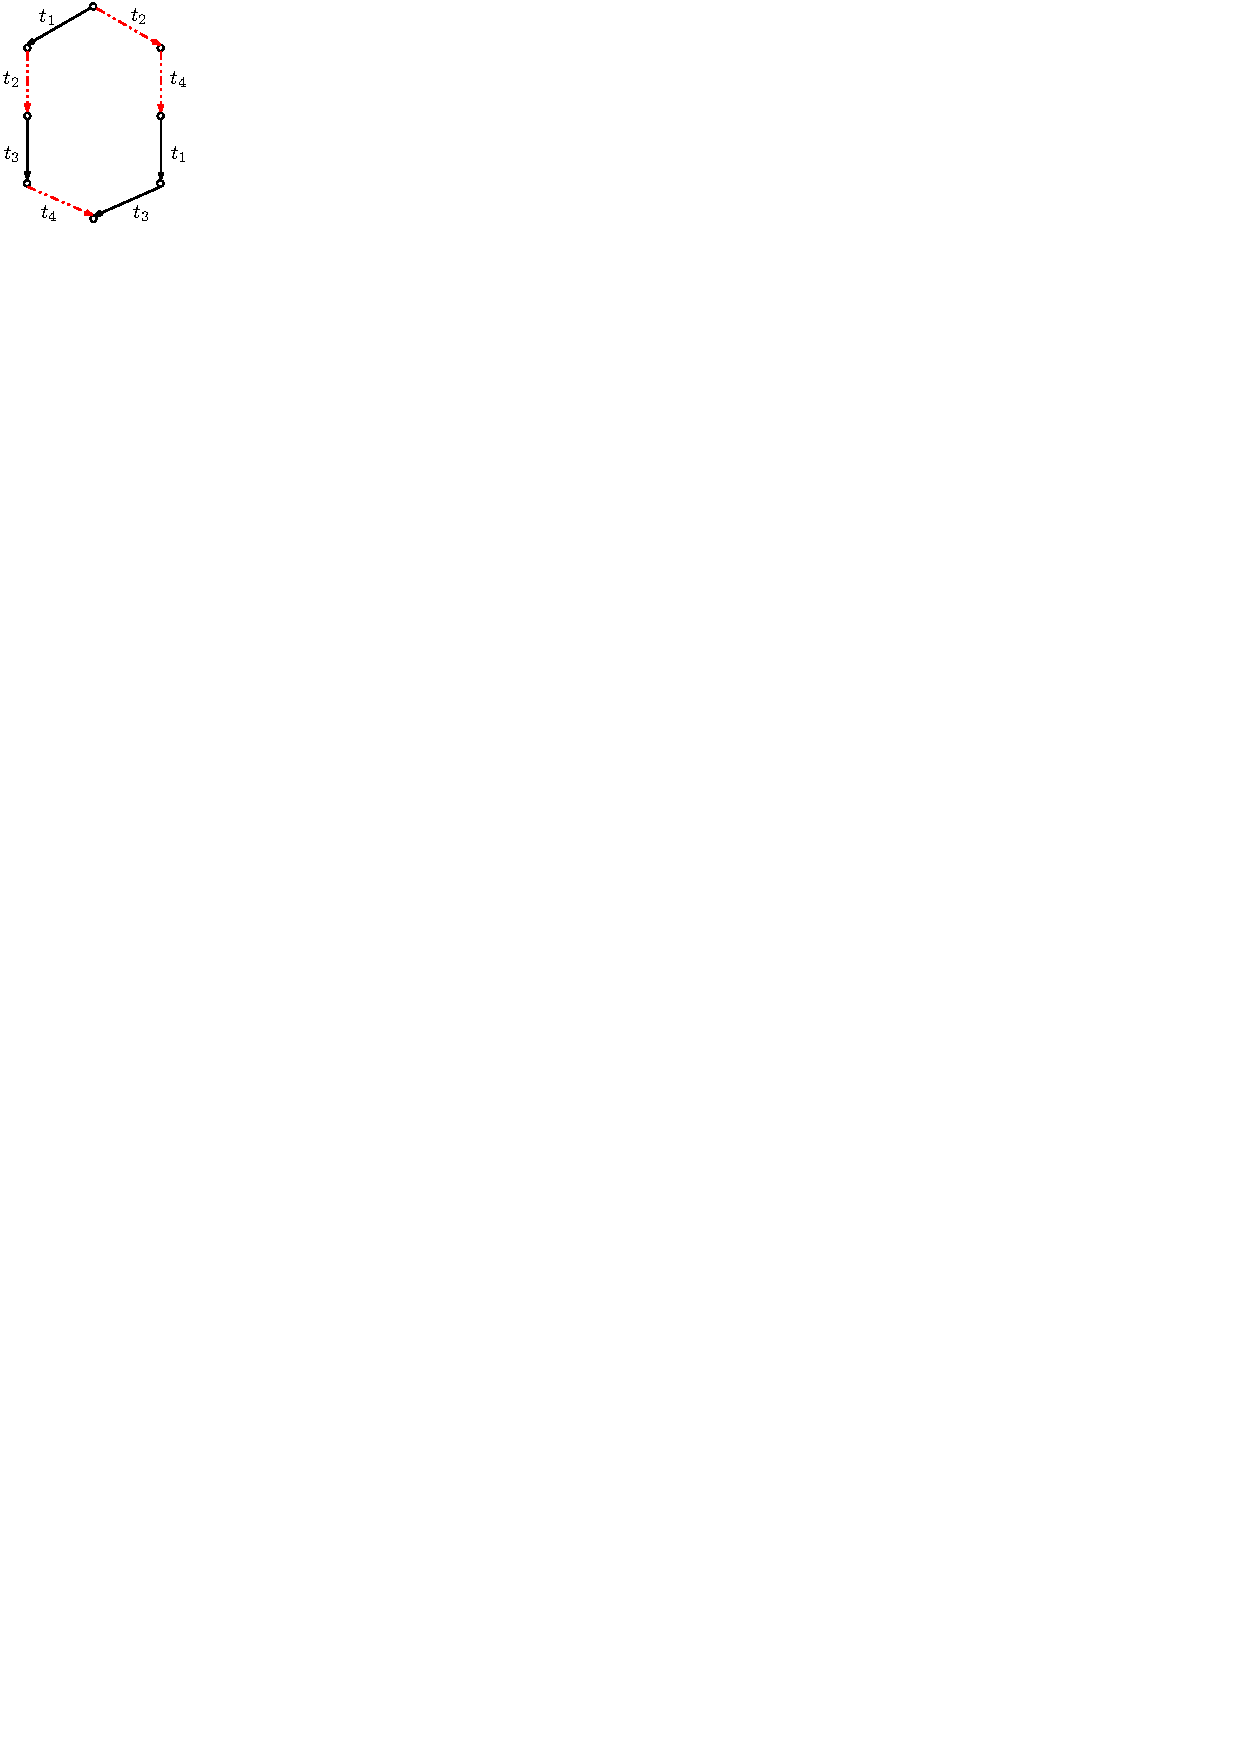
\includegraphics[height=3.5cm]{./img/rearrange}
        \caption{Rearranging Lemma %\\ (Lemma~\ref{lm:rearranging})
        }
        \label{fig:rearrange}
    \end{subfigure}
    \begin{subfigure}[b]{3.7cm}
    \centering
        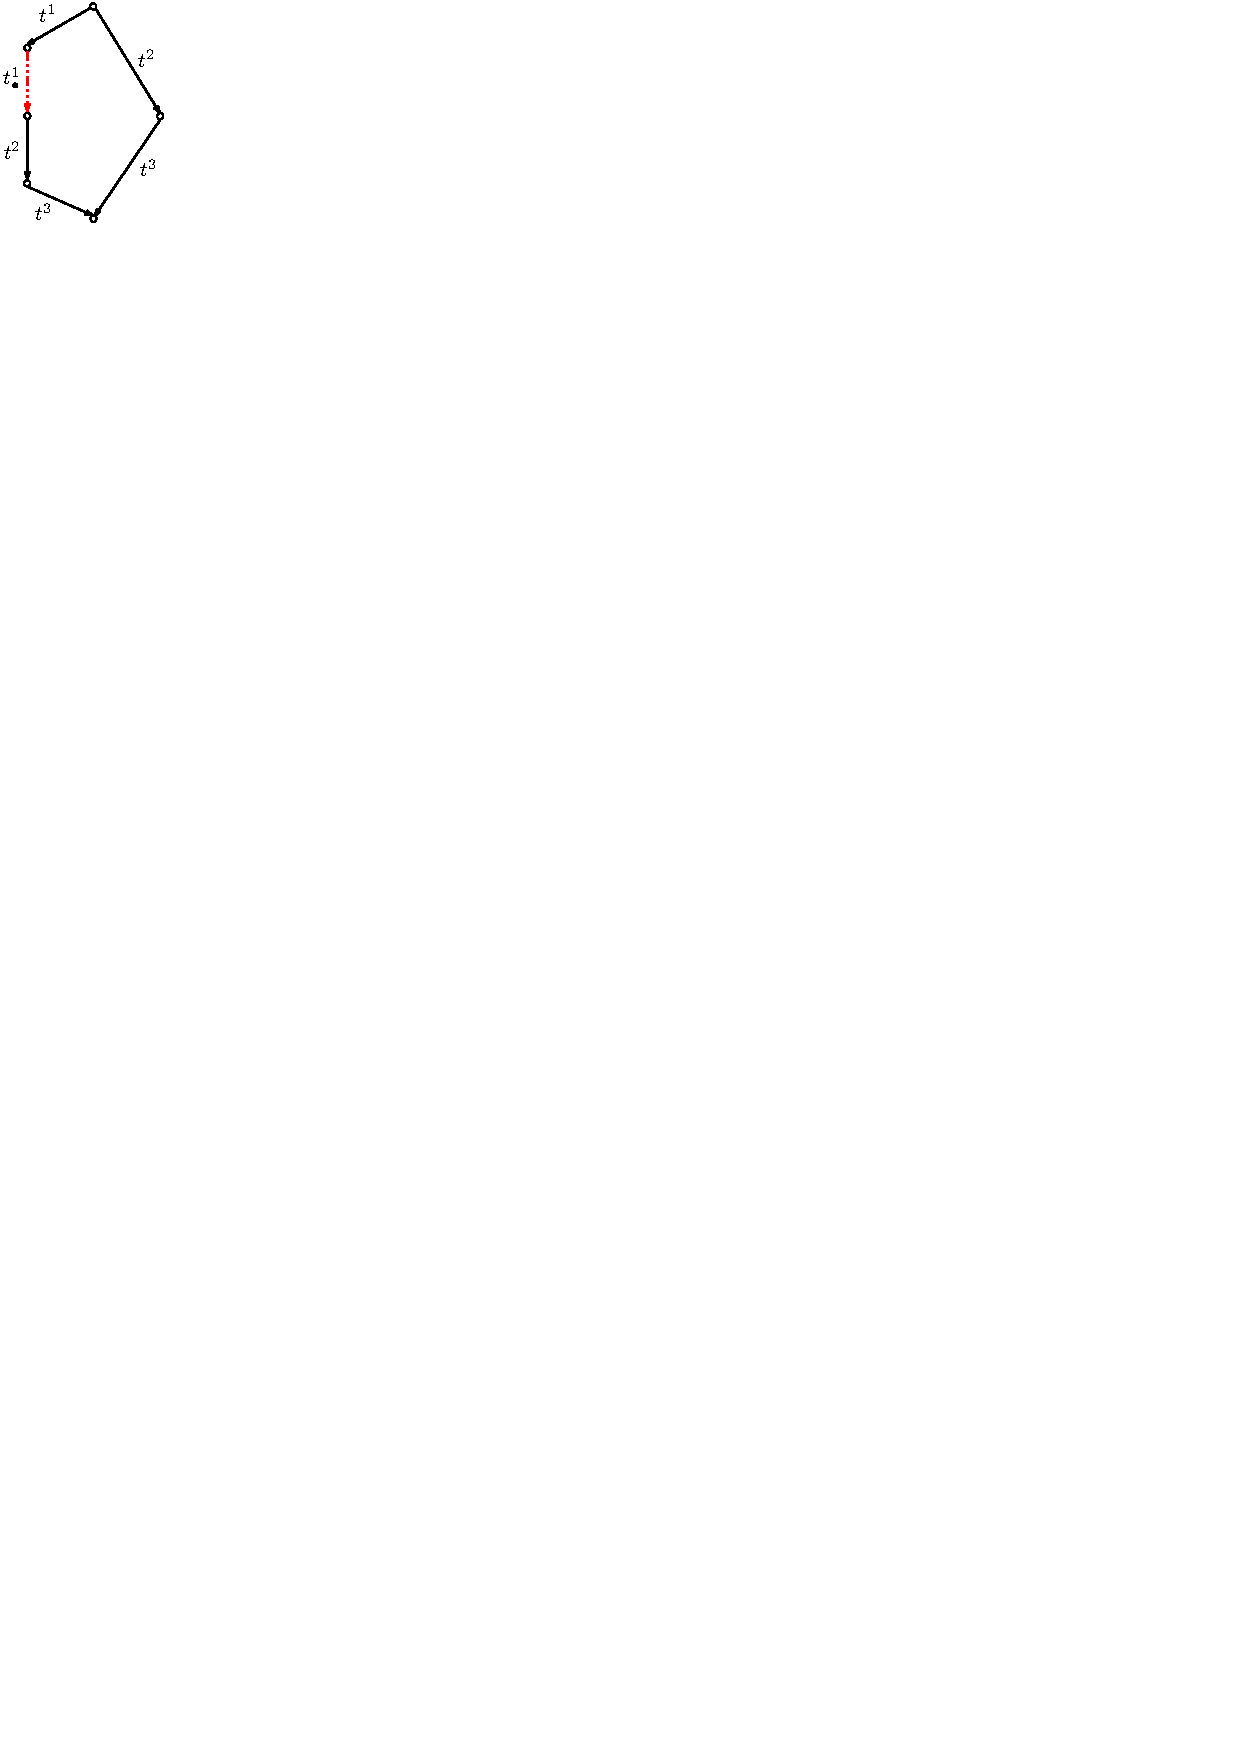
\includegraphics[height=3.5cm]{./img/short}
        \caption{Shortening Lemma %\\ (Lemma~\ref{lm:short})
        }
        \label{fig:short}
    \end{subfigure}
%    \caption{{%Graphical intuitions for the ingredients of the proof of causal consistency (Theorem~\ref{theo_caus}). 
%    Black, solid arrows represent forward reductions; red, dashed arrows represent backward reductions. 
%%    In (b), we assume that $t_{1}  \neq \rev{t_{2}}$, $t_{3}  \neq \rev{t_{2}}$, and $t_{3}  \neq \rev{t_{4}}$.
%}
%    }
    \end{figure}
    	\vspace{-5mm}
    {\small Black, solid arrows represent forward reductions; \\ red, dashed arrows represent backward reductions. }
	\end{frame}



%
%\begin{frame}
%	\frametitle{Chaining up the results}
%	\begin{enumerate}
%		\item first order choreographies are compliant with decoupled semantics
%		\item decoupled semantics is (weakly) bisimilar to atomic semantics
%		\item atomic semantics is causally-consistent
%	\end{enumerate}
%\end{frame}

\section{Final Remarks}
\begin{frame}
	\frametitle{Final Remarks}
	A process framework of reversible, multiparty asynchronous communication
	\bi
	\item built upon session-based concurrency
	\item flexible decoupled rollbacks
	\item causally consistent
	\ei 
	
	\bigskip
	
	\textbf{Future work}
	\bi
		%\item Improve the results with HO choreographies
		\item Add control to reversibility, via enhanced (monitor) types
			\begin{itemize}
				\item types with modalities
				\item types with logical conditions
			\end{itemize}
			Different monitors for the same process enact different behaviors 
		\item Compare with recent work on ``Concurrent Reversible Sessions''
		by Castellani, Dezani-Ciancaglini \& Giannini (CONCUR'17)
		\item Implement practical support for process specifications with reversibility (building upon CaReDeb)
		%Studying cost of reversibility (Tiezzi\&Yoshida, RC2016) 
	\ei
\end{frame}


\begin{center}
\maketitle
\end{center}
\end{document}

\begin{frame}
\frametitle{Global Semantics}

\begin{mathpar}
\inferrule*[left=\fwcolor{(FVal1)}]{}
{\ctx{G}[ \past \gtcom{p}{q}{U}{G}] 
\fwg 
\ctx{G}[\gtcom{p}{\!\!\past q}{U}{G} ]}
\\
\inferrule*[left=\bkcolor{(BVal1)}]{}
{\ctx{G}[\gtcom{p}{\!\!\past q}{U}{G} ]
\bkg
\ctx{G}[ \past \gtcom{p}{q}{U}{G}] 
}
\\
\inferrule*[left=\fwcolor{(FVal2)}]{}
{\ctx{G}[  \gtcom{p}{\!\!\past q}{U}{G}] 
\fwg 
\ctx{G}[\gtcom{p}{q}{U}{\past G} ]}

\\
\inferrule*[left=\bkcolor{(BVal2)}]{}
{
\ctx{G}[\gtcom{p}{q}{U}{\past G} ]
\bkg
\ctx{G}[  \gtcom{p}{\!\!\past q}{U}{G}] 
}
%\\
\end{mathpar}
\begin{itemize}
	\item Communications are two-staged: sending and receiving
	\item Labeled choices are easy to handle\footnote{Claudio A. Mezzina, Jorge A. P\'erez:
Causally Consistent Reversible Choreographies. CoRR abs/1703.06021 (2017)
}
\end{itemize}
\end{frame}

\begin{frame}
	\frametitle{Proof Tools}

	
	\begin{exampleblock}{Barb}
	$M\barb{\sred\p}$  if 
	$M\equiv \news{\vect n} (N \Par \np{\key{\loc}{\er}}{\conf{\stack C}{P}} \Par \moni{\ep{s}{\sred\p}}{ \ctx{S}[\past T] }{\mytilde x}{\store})$ where %
	$P\equiv \bout{\ep{s}{\sred\p}}{V}{Q} \Par R$ and $T=\ltout{\q}{U}{T_1}$.
\end{exampleblock}


A relation $\Re$ is a \emph{(weak) barbed bf simulation} if whenever $M \Re N$
\begin{enumerate}
	\item $M\barb{\p}$ implies $N\trans{\red}\barb{\p}$; 
	\item $M\fwa M_1$ implies $N\trans\fw N_1$, with $M_1 \Re N_1$; 
	\item $M\bka M_1$ implies $N\trans\bk N_1$, with $M_1 \Re N_1$.
\end{enumerate}

A relation $\Re$ is a  \emph{(weak) barbed bisimulation} if
 $\Re$  and  $\Re^{-1}$ are  weak bf barbed simulations.

\end{frame}

\begin{frame}
\frametitle{Result}

\begin{exampleblock}{Theorem 1}
Atomic semantics is causally consistent.
\end{exampleblock}

\begin{exampleblock}{Theorem 2}
For any atomically reachable configuration $M$, we have that $M \congruence\bfbw M$.
\end{exampleblock}

It suffices to show that the following relation is a 
bf weak bisimulation:
\begin{align*}
%	\Re =\{ (M,N) \st  M \trans{\fw} N \text{ via Rules~\fwcolor{(\textsc{Out})} \erase{or \fwcolor{(\textsc{Sel}})}} ~ \wedge   
%	\\
%M \trans{\bk} N \text{ via Rules~\bkcolor{(\textsc{ROut})} \erase{or \bkcolor{(\textsc{RSel}})}} \} 
	\Re =\{ (M,N) \st  M \trans{\fw} N \text{ via Rule~\fwcolor{(\textsc{Out})}} ~ \wedge 
	\\ 
	M \trans{\bk} N \text{ via Rule~\bkcolor{(\textsc{ROut})}} \} 
\end{align*}
\end{frame}

\begin{frame}
	\frametitle{Choreographies}
	If we restrain global type G to first order then:
	\begin{exampleblock}{}
Let $\mathsf{H}$  be a reachable, first-order global type with history \begin{enumerate}[a)]
\item If $\adeq{M}{\gth{H}}$ and $\gth{H} \fwg \gth{H}'$  then  $M \fw M'$  and $\adeq{M'}{\gth{H'}}$, for some $M'$.
%If $\adeq{M}{\gth{H}}$ and $\gth{H} \bkg \gth{H}'$ then $M \bkk M'$ (with $j =1$ or $j=2$) and $\adeq{M'}{\gth{H'}}$, for some $M'$.
 \item Suppose $\adeq{M}{\gth{H}}$. For all configurations $N_i$ such that $M \fw N_i$ there exist 
$\gth{H}_i, \gth{H}'_i, \gth{H}''$,
and $M'$,
such that
 $\gth{H} \swap \gth{H}_i\fwg \gth{H}'_i$,
 $\adeq{N_i}{\gth{H}'_i}$,
 $N_i \fws M'$,
 $\gth{H}'_i \fwgs \gth{H}''$,
 and 
 $\adeq{M'}{\gth{H}''}$
 (and similarly for $\bk$, $\bkg$).
\end{enumerate}
	\end{exampleblock}
	
\centering \blue{$\adeq{M}{\gth{H}} =$ $M$ is well-formed and implements $H$}	
\end{frame}

\begin{frame}
	\begin{definition}
We define $\causeq$ as the least equivalence between traces that is closed under composition and that obeys:
\begin{enumerate}[1.]
\item $t_1; t_2/t_1 \causeq t_2; t_1/t_2$; 
\item $t;\nottrace{t} \causeq \etrace_{\tsource{t}}$; 
\item $\nottrace{t};t \causeq \etrace_{\ttarget{t}}$.
\end{enumerate}
\end{definition}
\end{frame}

\end{document}